\newlength{\bibsep}
\documentclass[nonatbib,5p,a4paper]{elsarticle}  % 5p for two columns, 1p for 1 column (this is specific for the elsearticle)
\usepackage[english,norsk,nynorsk]{babel}        % Language
\usepackage[DatePublished]{Code/NTNU-lab}        % remove [DatePublished] to remove dates
\usepackage{csquotes}                            % Must be loaded when babel is loaded to avoid error.
% Use this file to write code that you do not want in the .sty file, but has to be in the preamble (before \begin{document}).
% Writing in this file in stead of in the preamble will keep the main file more organised and tidy.


%                       Nomenclatures
%_______________________________________________________________
\usepackage[intoc]{nomencl}
\makenomenclature

\renewcommand{\nomname}{%
% Title
%----------------
List of Symbols
%----------------
}
\renewcommand{\nompreamble}{%
% Description
%----------------
The next list describes several symbols that will be later used within the body of the document
%----------------
}
% This code creates the groups
\renewcommand\nomgroup[1]{%
  \item[\bfseries
  \ifstrequal{#1}{A}{Physics constants}{%
  \ifstrequal{#1}{B}{Mathematical constants}{%
  \ifstrequal{#1}{C}{Other symbols}{}}}%
]}
% This will add the units
\newcommand{\nomunit}[1]{%
\renewcommand{\nomentryend}{\\#1}}
%................................................................

                            % Write all preamble code in this file to keep it organised and tidy.

\addbibresource{Bibliography/Sources.bib}        % Selects the Bibliography file.


\begin{document}
\selectlanguage{english}                         % Sets the language of the document.

%%%%%%%%%%%%%%%%%%%%%%%%%%%%%%%%%%%%%%%%

\begin{frontmatter}
%
% Title:
%------------------------------------
\title{%
2022 PhD report\\
\small Planetary Model linking annd futur prospects  % A good idea is to have the subject code and name as subtitle
}
%
% Authors:
%------------------------------------
% List an author with name ' Firstname Middlename Lastname ' like this:
% F. M. Lastname
\author[Observatoire de Paris-Meudon]{C. Wilkinson} 
\author[Observatoire de Paris-Meudon]{B. Charnay}
\author[Observatory De La Côte D'azur]{S. Mazevet}
\author[Observatoire de Paris-Meudon]{AM. Lagrange}
\address[Observatoire de Paris-Meudon]{Obsrvatoire de Paris-Meudon - Lesia}
\address[Observatory De La Côte D'azur]{Observatory De La Côte D'azur}
%
% Date:
%------------------------------------
%
\newdate{dateName}{15}{07}{2022} % edit the date here, ' dateName ' has to match on these two lines.
\renewcommand*{\today}{\MonthYearDateFormat\displaydate{dateName}} 
% Options for displaying date: \MonthYearDateFormat,  \DayMonthYearDateFormat or \YearDateFormat
%
% Abstract:
%------------------------------------
\NameOfAbstract{Abstract} % Change abstract title here. If you write in Norwegian, write 'Sammendrag' (nb) or 'Samandrag' (nn)
\begin{abstract}
% Delete the text and write your abstract here:
%------------------------------------
To model the thermal evolution of Jupiter-like exoplanets and to link observational data with atmosphere and internal models, we build of two such models, Exorem and Exoris. We show that it is possible to link both atmosphere and interior models as to constrain the both and derive planetary parameters such as the internal energy flux, the radius and the spectral radiosity. We hence compute the parameters for a grid of models with varying internal and irradiation energy fluxes and masses. We show that our results are in agreement with that which is already published. We apply the combined model on the example of HD209458b where we can derive an internal temperature of 320K.\\
\\
"Numerical tools allow mediocre physicists like me to remain relevant in physics nowadays" S. Charnoz

\end{abstract}
%
\end{frontmatter}
%
%
% Table of contents:
%------------------------------------
% If the report is very long for some reason (over 4 or 5 pages), use a table of contents.
% Uncomment everything below the line ---- to get table of contents (ctrl + /) (the / on numberpad):
%-------------
%
% \ 
% \vspace{1cm}

% \begin{minipage}{\textwidth}
%     \tableofcontents
% \end{minipage}
% \clearpage
%% Prints a list of symbols. You can create/ change the categories in the preamble.tex file. 
% Learn more about nomenclature: https://www.overleaf.com/learn/latex/Nomenclatures
%
% Delete/change the text and write your Nomenclature here:
%------------------------------------

\nomenclature[A, 02]{\(c\)}{\href{https://physics.nist.gov/cgi-bin/cuu/Value?c}
{Speed of light in a vacuum}
\nomunit{\SI{299792458}{\meter\per\second}}}
\nomenclature[A, 03]{\(h\)}{\href{https://physics.nist.gov/cgi-bin/cuu/Value?h}
{Planck constant}
\nomunit{\SI[group-digits=false]{6.62607015e-34}{\joule\per\hertz}}}
\nomenclature[A, 01]{\(G\)}{\href{https://physics.nist.gov/cgi-bin/cuu/Value?bg}
{Gravitational constant} 
\nomunit{\SI[group-digits=false]{6.67430e-11}{\meter\cubed\per\kilogram\per\second\squared}}}
\nomenclature[B, 03]{\(\mathbb{R}\)}{Real numbers}
\nomenclature[B, 02]{\(\pi\)}{Pi}
\nomenclature[B, 01]{\(e\)}{Euler's constant}
\nomenclature[C]{\(V\)}{Constant volume}
\nomenclature[C]{\(\rho\)}{Friction index}

% Print statement:
%--------------------
\printnomenclature                 % List of symbols, can be useful
\section{Introduction}
% Delete the text and write your Introduction here:
%------------------------------------

Atmosphere models and interior models are often built separately and rely on two different underlying physical starting points. For the former, that atmospheres are in radiative convective equilibrium, and for the latter, that interiors are fully convective. However atmospheric models will, in most cases, give a convective profile for the deep atmosphere. Hence we can link these two separate models based on the premise that in such a region the physics are the same. The linkage of two separate models requires continuity of the four following quantities, temperature, pressure, gravity and mean molecular mass. This in itself leads to more of a mathematical and numerical problem then a physical one, should we start from the premise that there is indeed a space of parameters that leads to a solution. For the subsequent work we use the Exo-REM 1D radiatif convectif atmosphere model from the LESIA and the Exoris interior model from the Observatoire de la côte d'Azur. Atmosphere models come in many shapes and sizes but to accurately describe an atmosphere they need to posses a chemistry model preferably out of equilibrium, a cloud model and an parameterizable interior and exterior radiative flux. Exo-REM has the advantage of all of these aspects. However we shall not use the cloud model for the work presented here. Again interior models are plentiful, but fundamentally they need to use the best possible state equations of the elements that we might find inside a planet. Exoris contains such equations and one can change them as better ones come available. \par
One could wonder, what is the point in linking two distinct models? The answer to this question can be found in the internal radiative flux or conversly the internal temperature. It is hard to understand how one can fix this value in atmosphere models. For a gas planet of our solar system we can deduce it quite easily as we know the effective temperature and we know the stellar flux. However for a given gaseous exoplanet it is harder, especially so for irradiated planets where the effective temperature is mainly given by the stellar irradiation. Yet this internal temperature plays an important role in the atmospheres dynamics especially for young gaseous planets. Furthermore as a planet ages it evacuates internal energy, as such the internal temperature, in a sense, is a date stamp. As such we see the obvious conundrum, how do we access this internal temperature? The answer lies in the linkage of the models as stated, indeed if we can fix the thermal profile in the convective region of the atmosphere with an interior model, we can equally fix the internal temperature for a given set of planetary parameters. This will hence be the focal point of the subsequent work.


%% Place large figures that span the whole width of the page in here to easily move them around in the file
% and to avoid getting figures displayed after references and appendix. 
%
% Use {figure*} for a figure that will span both columns. 
% Below is an example of a figure with 6 sub-figures.
\begin{figure*}
%
        \subfigure[Contour plot number 1]{%
            \label{fig:Contour_1}
            \includegraphics[width=0.3\textwidth]{Images/Fig:Countour-plot/1-contour.pdf}
        }%
        \hspace{1em}
        \subfigure[Contour plot number 2]{%
            \label{fig:Contour_2}
            \includegraphics[width=0.3\textwidth]{Images/Fig:Countour-plot/2-contour.pdf}
        }%
        \hspace{1em}
        \subfigure[Contour plot number 3]{%
           \label{fig:Contour_3}
           \includegraphics[width=0.3\textwidth]{Images/Fig:Countour-plot/3-contour.pdf}
        }\\ %  ------- End of the first row ----------------------%
        \subfigure[Contour plot number 4]{%
            \label{fig:Contour_4}
            \includegraphics[width=0.3\textwidth]{Images/Fig:Countour-plot/4-contour.pdf}
        }%
        \hspace{1em}
        \subfigure[Contour plot number 5]{%
            \label{fig:Contour_5}
            \includegraphics[width=0.3\textwidth]{Images/Fig:Countour-plot/5-contour.pdf}
        }%
        \hspace{1em}
        \subfigure[Contour plot number 6]{%
            \label{fig:Contour_6}
            \includegraphics[width=0.3\textwidth]{Images/Fig:Countour-plot/6-contour.pdf}
        }%
%
    \caption{%
        Plots to be changed
     }%
   \label{fig:Countour-plot}
\end{figure*}                     % Change this to another line to move big figures.
\section{Atmosphere/Interior model description}
% Delete the text and write your Theory/ Background Information here:
%------------------------------------
% \parencite[131,136]{Griffiths}. for citations
% \footnotetext{I used this word as an umbrella term for variables, constants, vectors, tensors and other things that can be measured/ found empirically.} for footnotes.
% \dpd[order]{}{} = display mode partial derivative
\subsection{Exo-REM}

As stated previously, Exo-REM \parencite{baudino_interpreting_2015} is a 1D radiative convective model with an out of equlibrium chemistry model \parencite{baudino_toward_2017} and a cloud model \parencite{charnay_self-consistent_2018}. For completeness we shall describe the basic workings of such a model. The more informed reader can skip this part.\par
If we consider a cylindrical element of atmosphere of surface $dS$ and length $dl$ then light moving through this element will gain and lose intensity following the following subsequent expressions. 

\begin{align} % Use & sign to align, use \nonumber \\ to write a line without number.
    dI_{\lambda -} = -\kappa_{\lambda} I_{\lambda_0} dS \nonumber \\
    dI_{\lambda +} = \epsilon_{\lambda} dS
\end{align}

With $I_{0}$ the initial intensity before entering the element, $\kappa$ the absorption coefficient and $\epsilon$ the emission coefficient. Combining these two expressions we get the radiative transfer equation.

\begin{align}
    \frac{dI_{\lambda}}{dS} = -\kappa_{\lambda} I_{\lambda} + \epsilon_{\lambda} \label{eq:pre-RTE}
\end{align}

\Cref{eq:pre-RTE} % Use \Cref at the start of a sentence and \cref mid sentence.
can be rewritten using the extinction coefficient $\tau$, which corresponds to the inverse of the average distance traveled by a photon before being scattered, whose expression is given by :

\begin{align}
    \tau_{\lambda} = \int \kappa_{\lambda} dS
\end{align}

As well as the source function given by :

\begin{align}
    S_{\lambda} = \frac{\epsilon_{\lambda}}{\kappa_{\lambda}}
\end{align}

Considering an atmosphere in local thermodynamic equilibrium defined as :

\begin{align}
    S_{\lambda} = B_{\lambda}
\end{align}

With B the idealized black body profile. we can hence write \cref{eq:pre-RTE} as :\par

\begin{align}
    \frac{dI_{\lambda}}{d\tau_{\lambda}} = -I_{\lambda} + B_{\lambda}
\end{align}

The absorption coefficient is in reality a sum of different contributions to the absorption of a parcel of atmosphere :

\begin{align}
    \kappa_{\lambda} = \kappa_{\lambda, chemistry} + \kappa_{\lambda, Rayleigh} + \nonumber \\
    \kappa_{\lambda, pair} + \kappa_{\lambda, aerosol}
\end{align}
With the various contributions defined as follows :\par
\begin{itemize}
    \item {$\kappa_{\lambda, chemistry}$} : Absorption by atoms/\\molecules.
    \item {$\kappa_{\lambda, Rayleigh}$} : Light scattered by \\fine particles.
    \item {$\kappa_{\lambda, pair}$} : Collision induced scattering.
    \item {$\kappa_{\lambda, aerosol}$ : Scattering, absorption due to\\ aerosols.}
\end{itemize}

While the specificity's of each of these coefficients is beyond the scope of the intended purpose of this work it is important to understand the expression of $\kappa_{\lambda, chemistry}$ to understand how Exo-REM links radiative transfer, chemistry and temperature profile. It's value is given by the following expression :

\begin{align}
    \kappa_{\lambda, chemistry} = \sum_{i=1}^{N_{species}} n_{i} \sigma_{\lambda,i}
\end{align}

With $N_{species}$ the molar concentration of species $i$ and $\sigma_{\lambda,i}$ the cross section which corresponds to the capacity to absorb at a given wavelength it is temperature and pressure dependant. Extensive experimental work is required to determine the values of cross sections. A humble physicist should keep in mind that the theoretical models used are only as good as the underlying experimental data and these values require updating regularly.\par

Resolving the radiative transfer equation at different levels (conversely optical depths) of the atmosphere does not suffice as we lack here the mechanical properties of layers of atmospheres at different thermodynamic conditions sat upon one another. Atmospheres on an averaged large scale can be quite accurately modeled using the hydrostatic balance equations linking mass $M$, pressure $P$, radius $r$, density $\rho$ using the universal gravitational constant $G$, which can be expressed as follows : \par

\begin{align}
    \frac{P}{dr} = -\frac{GM\rho(r)}{r^{2}} \label{eq:HBE}
\end{align}

The density $\rho$ here is linked to the temperature $T$, pressure $P$, mass $M$ using the ideal gas constant $R$, via the ideal gas law expressed as follows :

\begin{align}
    P = \frac{\rho R T}{M} \label{eq:IG}
\end{align}


The most attentive readers at this point might have alarm bells ringing as we mention deep atmosphere in the introduction where this law will hold up badly. This will be mentioned further in a subsequent section.\par

The fluxes considered in the radiative transfer equation are that of the stellar irradiation and the internal energy. They shall be subsequently expressed in temperatures using the Stefan Boltzmann approximation as shown in \cref{eq:SB}

\begin{align}
    \int_{0}^{\infty} \frac{\hbar}{4\pi^2c^2}\frac{\omega^3}{e^{\frac{\hbar\omega}{k_B T}}-1}\, d\omega = \sigma T^4 \label{eq:SB} \\
    \sigma = \frac{k_B^4}{4\pi^2c^2\hbar^3}\frac{\pi^4}{15} \nonumber
\end{align}

As such with the stated ingredients, it is possible to build a 1D atmosphere model like Exo-REM. Further physical aspects \parencite{charnay_self-consistent_2018} and the precise resolution method are beyond the current scope of this work but will be detailed in subsequent work. 

\subsection{Exoris}

As stated in the introduction, Exoris helps resolve the internal structure of a planet and relies on a library of equations of state. The range of parameters inputted into Exoris are give in \cref{tab:Exrs}.\par

\begin{table}[htb]%
\centering
\caption{Exoris parameters.}
	\label{tab:Exrs}
	\begin{tabular}{c}
		\toprule
		{$Exoris$}  \\
		\midrule
        \midrule
        {Mass of planet} \\
        \midrule
		{Mass fraction of core}   \\
        \midrule
		{Helium to hydrogen mass ratio}   \\
        \midrule
		{Water mass fraction}   \\
        \midrule
		{Proportion of rock in the core}   \\
        \midrule
        {Equation(s) of state for envelope}   \\
        \midrule
        {Equation(s) of state for core}   \\
        \midrule
        {Equation of state for ice}   \\
        \bottomrule
	\end{tabular}
\end{table}

Exoris seeks to solve the hydrostatic balance equation \cref{eq:HBE} using no longer the ideal gas law \cref{eq:IG} but rigorous equations of state (EOS) where the state of the considered matter varies depending on the pressure considered. To accomplish this, Exoris considers an adiabatic profile, where the entropy is defined by the helium to hydrogen mass fraction in the envelope at an initial "surface pressure".

\begin{align}
    S*n_{tot} = S_{h}*n_{h} + S_{he}*n_{he} + S_{mix}\label{eq:S1}
\end{align}

With $n_x$ the number of moles of each species and $S_{mix}$ the non linear mixing term. In practice we neglect $S_{mix}$ when estimating the adiabat. When using the mass fraction of helium $\gamma_{He}$, \cref{eq:S1} becomes :

\begin{align}
    S = S_{h}\frac{4-4\gamma_{He}}{4-3\gamma_{He}} + S_{he}\frac{\gamma_{He}}{4-3\gamma_{He}} \label{eq:S2}
\end{align}

It is also necessary to compute the "surface density" from the pressure and temperature conditions.

\begin{align}
    \frac{1}{\rho} = \frac{\alpha_H}{\rho_He} +  \frac{\alpha_{He}}{\rho_{He}} +  o(\delta V) \label{eq:D1}
\end{align}

Again here we will neglect mixing terms. Substituting the helium to hydrogen mass fraction ($\gamma_{He}$) into \cref{eq:D1} we get :

\begin{align}
    \rho = \frac{\rho_H*\rho_{He}}{\gamma_{He}*\rho_H + (1-\gamma_{He})*\rho_{He}} \label{eq:D2}
\end{align}

Once the planets entropy is fixed it is possible to determine the pressure temperature profile along a pressure grid by supposing that the system is adiabatic. Hence it is possible to derive a density profile and using \cref{eq:HBE} a radial profile. However it is necessary to take into account the different compositions within the planet and most notably the core. To do this, once an initial profile is constructed, the boundary for the core can be placed using the core mass fraction specified by the user. Doing so leads to Exoris reevaluating the temperature and density profile taking into account a new domain with a change of EOS, which will in turn lead to an adjustment of the boundary for the EOS change. Iterating this process a certain number of times leads to a converged profile which abides by the input parameters.\par

The EOS used by exoris for the hydrogen helium enveloppe is the S. Chabrier et al. 2019 updated dense hydrogen–helium mixtures EOS \parencite{chabrier_new_2019}. Benchmarks of the results produced with Exoris were done using the 1995 Saumon et al. SCVH equations \parencite{saumon_equation_1995}. \Cref{fig:M-R_benchmark},  where the underlying data is from Militzer et al. \parencite{militzer_ab_2013}, compares the two EOS, we chose to test various "surface pressures" in order to determine the impact that the inital entropy has on the outcome. We see that differences appear for high entropies (high temperature) and most notably at low mass. This diagram shows the intrinsic challenge of comparing models to one another which use different EOS. One has to be cautious. \par

\begin{figure}
    \centering
    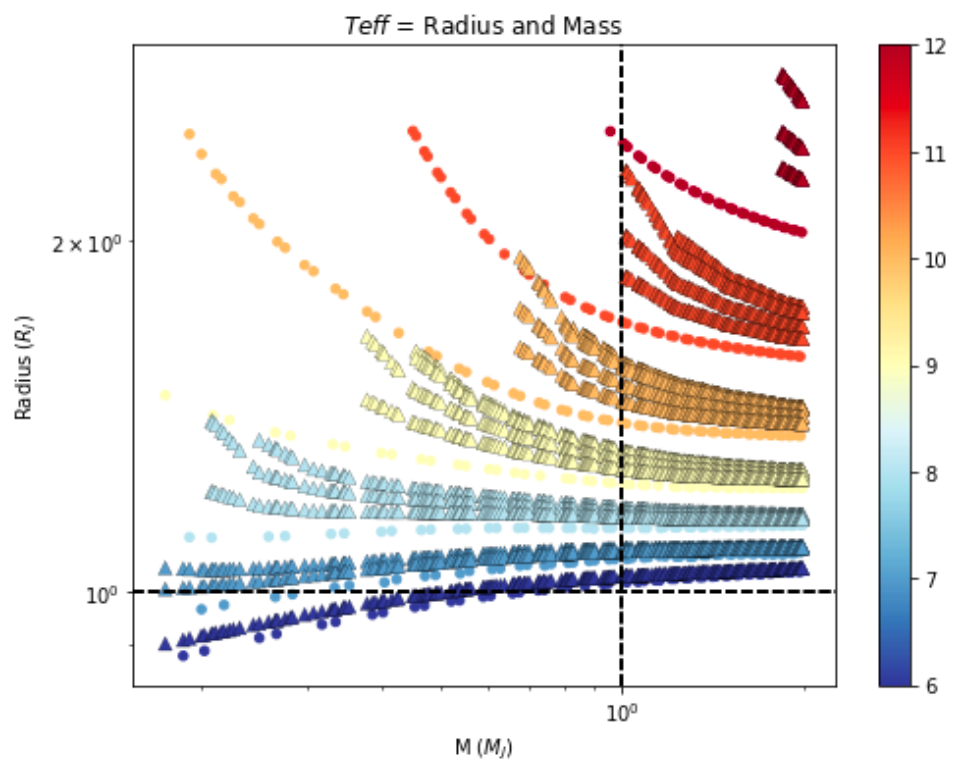
\includegraphics[width=0.48\textwidth]{Images/M-R_benchmark.png}
    \caption{Mass radius diagramme comparing Chabrier et al. 2019 (triangles) vs Saumon et al. 1995 circles with entropy on color axis in $K_b/el/mol$, multiple curves for different "surface pressures").}
    \label{fig:M-R_benchmark}
\end{figure}

Rigorous EOS are not plenteous and combining EOS is physically dubious as non linear terms that can have a strong impact are often neglected. In order to emulate higher atomic number compositions it is standard to increase the molecular concentration of other elements than hydrogen. In our case this would be H2O. We show how this is done in \cref{eq:compo} where $Z_m$ corresponds to higher atomic number elements.

\begin{align}
    \label{eq:compo}
    X_h + Y_{He} + Z_{H_2O} + Z_m = 1 \nonumber \\
    X_h + Y_{He} + Z'_{H_2O} = 1 \\ 
    with \,\,  Z'_{H_2O} = Z_{H_2O} + Z_m \nonumber 
\end{align}

By doing this, we need to change \cref{eq:S1} and \cref{eq:S2} to account for the added water in the envelope. We hence obtain the following equations :

\begin{align}
    S*n_{tot} = S_{H}n_{H} + S_{He}n_{He} + S_{He}n_{H_2O} + S_{mix}\label{eq:S3}
\end{align}

Again neglecting the ideal mixing term and using the helium to hydrogen mass fraction ($\gamma_{He}$) and water mass fraction ($\gamma_{H_2O}$), we obtain the following expression for $S$ :

\begin{align}
    x_h = \frac{36*(\gamma_{H_2O}-1)*(\gamma_{He}-1)}{\gamma_{H_2O}*(27*\gamma_{He}-34)-27*\gamma_{He}+36} \nonumber \\
    x_he = -\frac{9*(\gamma_{H_2O}-1)*\gamma_{He}}{\gamma_{H_2O}*(27*\gamma_{He}-34)-27*\gamma_{He}+36} \nonumber \\
    x_h2o = \frac{2*\gamma_{H_2O}}{\gamma_{H_2O}*(27*\gamma_{He}-34)-27*\gamma_{He}+36} \nonumber \\
    S = S_{h}x_{H} + S_{he}x_{He} + S_{he}x_{H2O} \label{eq:S4}
\end{align}

Again we need to compute the "surface density" and the given pressure and temperature conditions. We hence add the density term for water onto \cref{eq:D1} and again neglecting mixing terms, we get :

\begin{align}
    \frac{1}{\rho} = \frac{\alpha_H}{\rho_He} +  \frac{\alpha_{He}}{\rho_{He}} +  \frac{\alpha_{H_2O}}{\rho_{H_2O}} \label{eq:D3}
\end{align}

Again here we will neglect mixing terms. Substituting he helium to hydrogen mass fraction ($\gamma_{He}$) and water mass fraction ($\gamma_{H_2O}$) into \cref{eq:D3} we get : 

\begin{align}
    \rho = \frac{rho_H*rho_{He}*rho_{H_2O}}{(\rho_H*\rho_{He}*\gamma_{H_2O}-\rho_H*\rho_{H_2O}*(\gamma_{H_2O}-1)*\gamma_{He}+\rho_{He}*\rho_{H_2O}*(\gamma_{H_2O}-1)*(\gamma_{He}-1))} \label{eq:D4}
\end{align}

Nullifying $\gamma_{H_2O}$ in \cref{eq:S4} and \cref{eq:D4} gives as expected \cref{eq:S2} and \cref{eq:D2}. Details on how \cref{eq:S4} and \cref{eq:D4} are derived are given in the annexes. Details on the derivation of $S_{mix}$ are equally given in the annexes.

Exoris is also capable of evaluating the gravitational moments but this is beyond the scope of this work.

\section{Joined model method}
% Delete the text and write your Method(s) here:
%------------------------------------
In the subsequent section we shall in detail describe the method used to link the atmosphere and interior model. \Cref{tab:QOI} details the quantities that will be used.\par

\begin{table}[htb]%
\centering
\caption{Quantities of interest.}
	\label{tab:QOI}
	\begin{tabular}{ccc}
		\toprule
		Variable & {Exorem}  &  {Exoris}  \\
		\midrule
        \midrule
        Pressure & {$P_{rem}$}  &  {$P_{ris}$}  \\
        \midrule
		Temperature at 1bar & {$T_{rem}$}  &  {$T_{ris}$}  \\
        \midrule
		Mass at 1bar & {$M_{rem}$}  &  {$M_{ris}$}  \\
        \midrule
		Radius at 1bar & {$R_{rem}$}  &  {$R_{ris}$}  \\
        \midrule
		Gravity at 1bar & {$g_{rem}$}  &  {$g_{ris}$}  \\
        \midrule
		Molar mass at 1bar & {$\mu_{rem}$}  &  {$\mu_{ris}$}  \\
        \midrule
		Variable (X) at P & {$X_{rem}(P)$}  &  {$X_{ris}(P)$}  \\
        \midrule
		Internal temperature & {$T_{int}$}  &  {-}  \\
        \midrule
		Irradiation temperature & {$T_{irr}$}  &  {-}  \\
        \midrule
		{Variable (X) at $P_c$} & {$X_{rem-c}$}  &  {$X_{ris-c}$}  \\
        \midrule
		Convective region & {$P_c$}  &  {-}  \\
        \midrule
		Entropy & {-}  &  {$S$}  \\
        \midrule
		Core mass ratio & {-}  &  {$core$}  \\
        \midrule
		He/H fraction & {-}  &  {$\gamma_{he}$}  \\
		\bottomrule
	\end{tabular}
\end{table}

It is inherently hard to link very different models and a certain amount of choices and approximations need to be made, they are as follows :

\begin{itemize}
    \item Model linkage can only be done at pressures where the atmosphere is convective
    \item The mass of the atmosphere is considered negligible compared to that of the interior and core
    \item The atmosphere's mean molecular weight is reached in the interior by adjusting the He/H fraction
\end{itemize}

We also need to know what quantities absolutely need to be linked, they are as follows :

\begin{itemize}
    \item Pressure
    \item Temperature
    \item Molecular mass
    \item Gravity
\end{itemize}

One could expect it to be necessary to link the heat capacity ratio which is defined as follows :\par

\begin{align} 
    \frac{\partial ln(T)}{\partial ln(P)} = \frac{\gamma - 1}{\gamma} \Bigg|_{S} \label{eq:HC}
\end{align}

However as we are considering linking two models with different equations of state this is not deemed possible and also unnecessary. Indeed should pressure, temperature and molecular mass be equal then the heat ratio will be continuous too. (To be verified)\par

To guide the linkage a grid of both models is made over a range of input values, the grid is explicited in \cref{tab:Exorem} and \cref{tab:Exoris}

\begin{table}[htb]%
\centering
\caption{Exorem grid layout.}
	\label{tab:Exorem}
	\begin{tabular}{c}
		\toprule
		{$exorem(T_{int},T_{irr},g_{rem}) = T_{rem}(P), \mu_{rem}(P), P_c$}  \\
		\midrule
        \midrule
        $T_{irr} \in [0;1500] \, (K)$ \\
        \midrule
		$T_{int} \in [0;1000] \, (K)$   \\
        \midrule
		$g_{rem} \in [2;100] \, (m/s^2)$   \\
        \bottomrule
	\end{tabular}
\end{table}

\begin{table}[htb]%
\centering
\caption{Exoris grid layout.}
	\label{tab:Exoris}
	\begin{tabular}{c}
		\toprule
		{$exoris(T_{ris},core,\gamma_{he/h}, M) = S, R_{rem}$}  \\
		\midrule
        \midrule
        {$T_{ris} \in [150;1500] \, (K)$} \\
        \midrule
		{$core = 10 \, M_{e}$}   \\
        \midrule
		{$\gamma_{he} \in [0.1;0.5]$}   \\
        \midrule
		{$M \in [0.1;15] \, (M_J)$}   \\
        \bottomrule
	\end{tabular}
\end{table}


Given grid parameters depend on the capacity of the models to converge correctly, low temperature inputs can lead to non converged solutions. \par

\begin{figure}
    \centering
    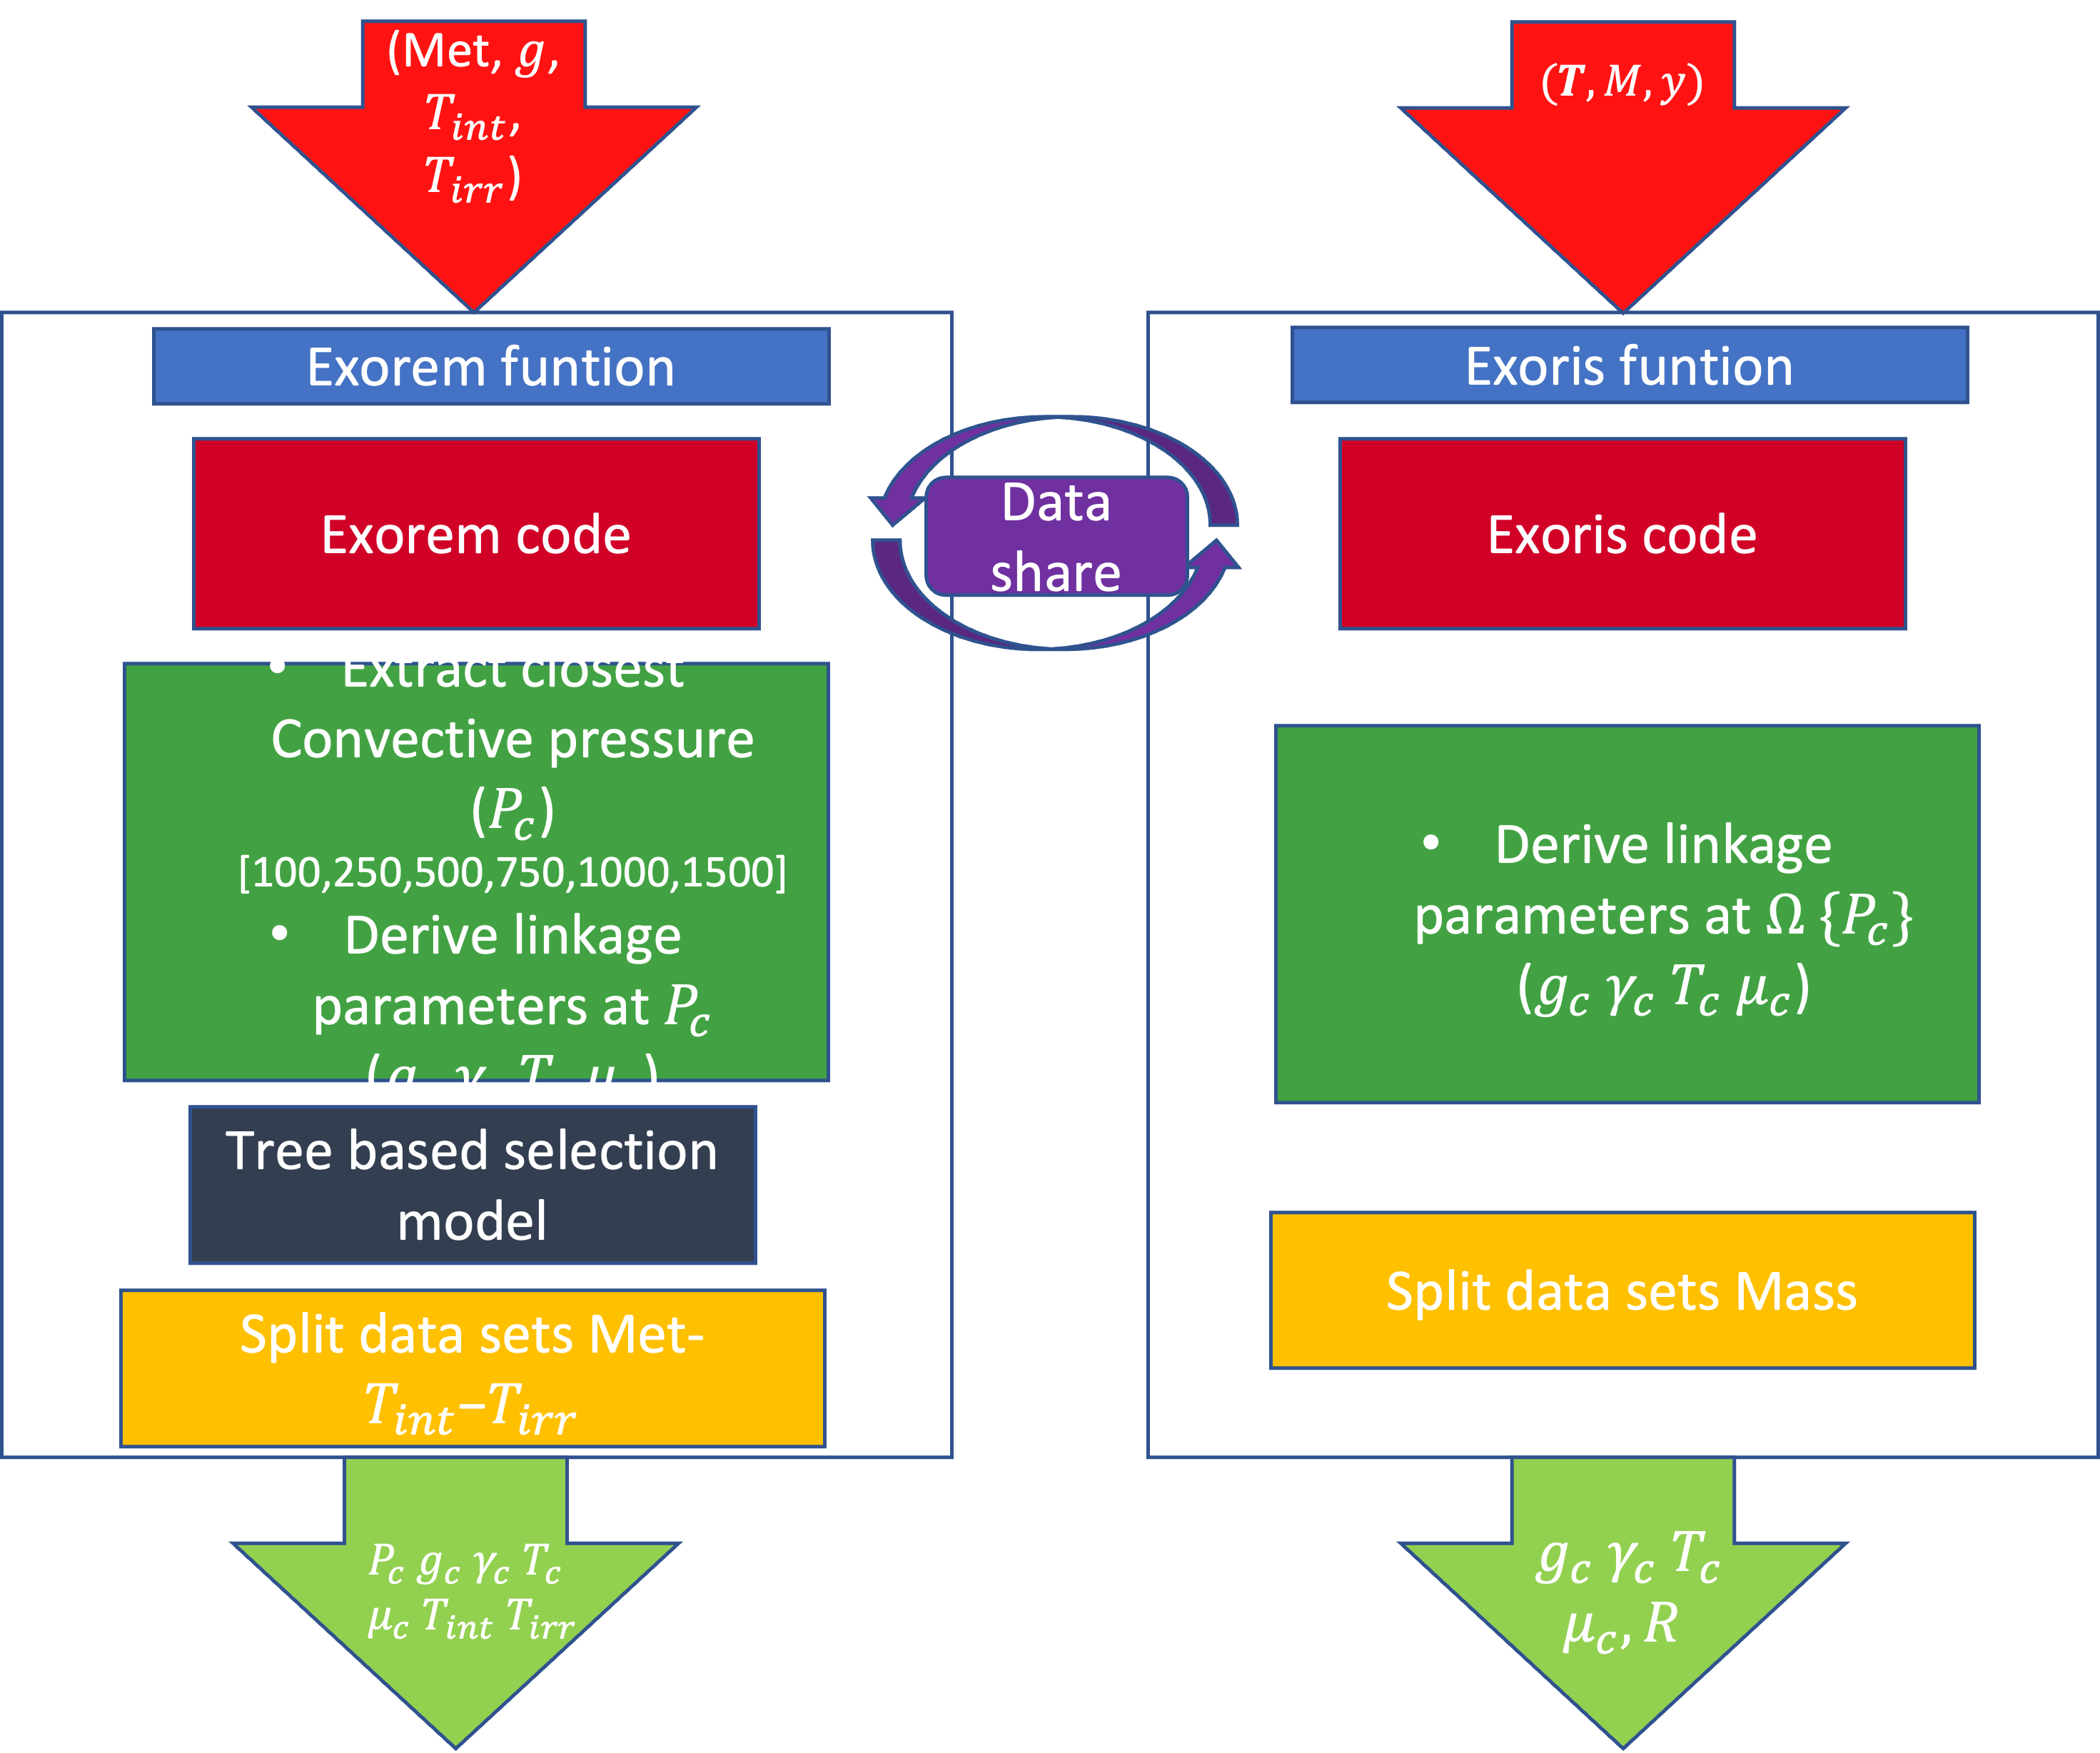
\includegraphics[width=0.48\textwidth]{Images/grid_model_function.png}
    \caption{Organigram of how Exoris and Exorem are packaged into grid functions.}
    \label{fig:Exoris_Exorem_grid_functions}
\end{figure}

\Cref{fig:Exoris_Exorem_grid_functions} details how exorem and exoris grids are in practice made. To help subsequent steps, there is a small level of grid sharing on tempereature values between exorem and exoris. This is to make sure that the grids overlap. Exorem can struggle to converge at low irradiation temperatures for high internal temperatures. A non grey analytical model from Guillot \parencite{guillot_radiative_2010} is used in these regions to initialise exorem with pressure temperature profiles. However, this is often not sufficient, as such, a basic tree based machine learning model is trained to remove improperly converged pressure-temperature profiles, further details can be found in the anexes. \par

Linkage between models is always carried out for the pressures where Exorem is convective, this adds a certain level of complexity to the problem. Indeed to minimize the effect of the non-precise ideal gas law used in exorem, we want to link at the lowest possible pressure as such at the point where the atmosphere has started exhibiting a convective behaviour. We hence need to interpolate the exoris quantities to this pressure. In practice we avoid doing this as it would be computationally tiresome and would lead to the size of the exoris grid being multiplied by the size of the exorem one. As such the convective pressures for all the exorem grid values are grouped into a bins of convective pressures. These bins are 100, 250, 500, 750, 1000 and 1500 bars, the bin is chosen as to always be of a superior value to the real convective pressure as to insure that the atmosphere is indeed convective. \par

Using the grids as a guide, the linkage is done via iterative calling of the exorem and exoris code. As shown in \cref{fig:Exoris_Exorem_grid_functions} we split the grids into $T_{int}$ and $T_{irr}$ sub grids for exorem and $M_{ris}$ subgrids for exoris. Hence the process outlined in \cref{fig:Iterative_process} is undertaken for a user chosen ($T_{int}$,$T_{irr}$,$M_{ris}$,$core$) where $M_{ris}$ will become the chosen planatary $M$ for which we wish to determine the properties such as the radius ($Req$), spectra ($J_{rad}$), effective temperature ($T_{eff}$) and entropy ($S$).\par

\begin{figure}
    \centering
    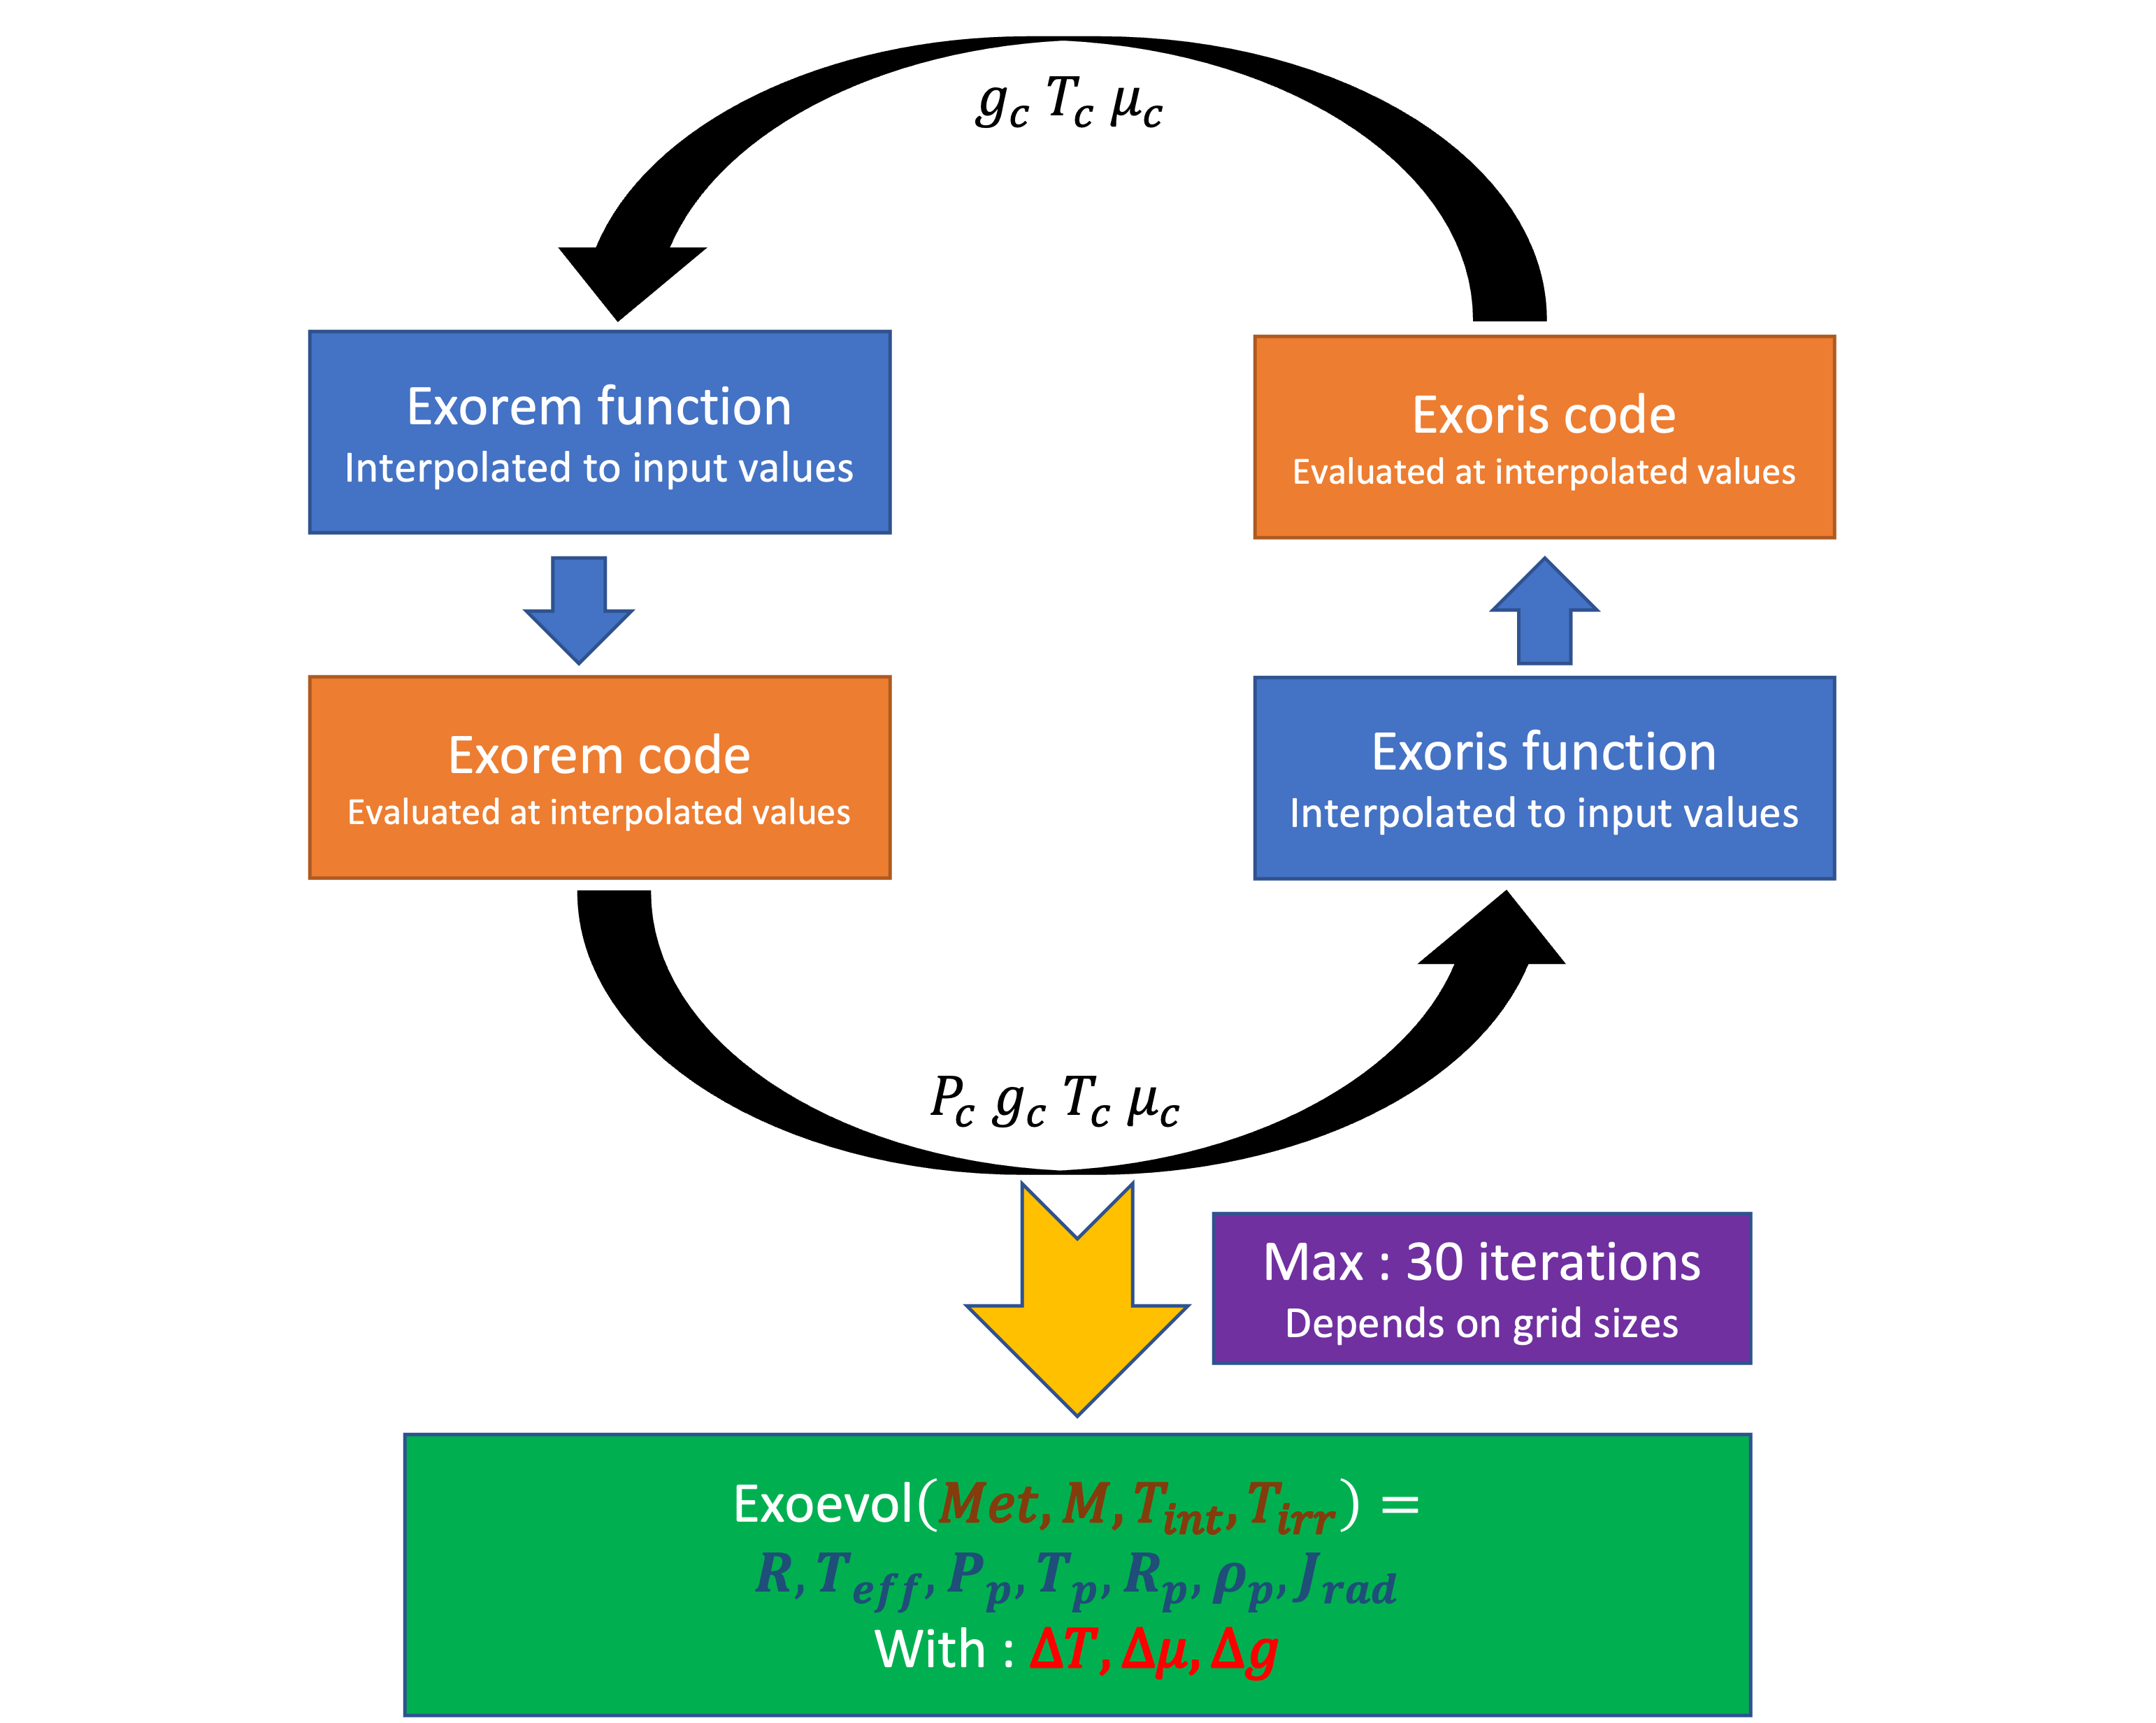
\includegraphics[width=0.48\textwidth]{Images/Iterative_process.png}
    \caption{Iterative process to converge exorem and exoris models}
    \label{fig:Iterative_process}
\end{figure}

The objective of this iterative process is to reduce the erreur on the three quantities to link below a certain threshold. This threshold is determined a posteriori as to find the right balance between convergence time and precision.\par

It is worth detailing the interpolation method in order to understand better the steps completed during an iteration. Interpolation in high dimensional space poses notable challenges. Indeed points can be distant from one another and desired points can be badly surrounded by grid values. It is important to know the layout of the variables and what we want to obtain. Using the details from \cref{tab:Exorem} and \cref{tab:Exoris}, we see the input and output variables. Input variables are always given at a pressure of 1 bar and output variables at the linkage pressure ($P_c$). As such as stated, before running the iterative procedure including interpolations, we have fixed ($T_{int}$,$T_{irr}$,$M_{ris}$,$core$). We hence need to find at each step ($g_{rem}$,$T_{ris}$,$\gamma_{he}$) from the values obtained at the linkage pressure ($P_c$,$T_c$,$\mu_c$,$g_c$). We will seperate the cases between exorem and exoris.\par

For exorem, we uniquely need to find the equatorial gravity at 1bar, to do this a simple plotting of how the surface gravity varies with the given parameters shows the following :

\begin{align} 
    g_s = f(P_c,T_c,\mu_c,g_c) = f(P_c, g_c) \overset{\mathrm{at \, P_c}}{=} ag_c + b \\
    (a,b) \in (R,R) \nonumber
\end{align}

As such we use a simple linear regression. We avoid all extrapolations. As such, should the value of $g_c$ not be included in the grid, then an exploration is undertaken as to include it. This can be the case for large mass planets.\par

For exoris, we need to find $T_{ris}$ and $\gamma_{He}$. To do this we chose to fix the input value of $\gamma_{He}$ using the average molecular mass ($\mu_c$) using the following :

\begin{align} 
    \frac{1}{\mu_c} = (1-\gamma_{He})\frac{1}{\mu_{H_2}} + \gamma_{He}*\frac{1}{\mu_{He}}
\end{align}

Which gives $\gamma_{he}$ :

\begin{align} 
    \gamma_{He} = 2-\frac{4}{\mu_c}
\end{align}

However the $\gamma_{He}$ here is evaluated using exorem, as such we need to be cautious. In exorem one mol of atmosphere contains a mix of the potential chemicals of interest including $H_2$ and not atomic hydrogen as is used in the mass ratio for exoris, we hence need to define this evaluated $\gamma_{He}$ as $\gamma_{He}^*$ which is defined as follows.

\begin{align} 
    \gamma_{He}^* = \frac{m_{He}}{m_{H_2}+m_{He}}
\end{align}

In exoris we have  $\gamma_{He}$ defined as :

\begin{align} 
    \gamma_{He} = \frac{m_{He}}{m_{H}+m_{He}}
\end{align}

The reason behind this difference is due to the EOS for hydrogen which is standardized for $H$.

As such if we use $m_H = m_{H_2}/2$ we have the following expression for  $\gamma_{He}$ in exoris :

\begin{align} 
    \gamma_{He} = \frac{2\gamma_{He}^*}{\gamma_{He}^*+1}
\end{align}

We can now look for the surface pressure to use in exoris ($T_{ris}$). To do this, we again plot its behaviour against the given parameters at $P_c$ this shows the following :

\begin{align} 
    T_{ris} = f(P_c,T_c,\mu_c,g_c) \overset{\mathrm{at \, P_c}}{=} f(T_c,\mu_c,g_c)
\end{align}

Indeed this represents a certain challenge as $T_{ris}$ is the result of a combination of all the parameters. We hence have to interpolate in a four dimensional space. To do this we propose to use a barycentric interpolation using a Delaunay triangulation, the full description of this method is given in the annexes. From a practical standpoint, this method requires the desired point to be contained within a triangle (pyramid in 3d). Either this is already the case with the guiding grid and a point within the triangle can be found, or this is not the case and an exploration is required to build the surrounding values. It is uncertain how smooth the space included within the triangulation values is. As such multiple iterations of interpolation and exoris model running are required in order to find the point of interest within a given tolerance. \par

These interpolation and model running steps are shown in \cref{fig:Iterative_process}. More work is required for the interpolations, most notably how to find surrounding values efficiently.

(Image showing convergence evolution required here)
\section{Results}
% Delete the text and write your Results here:
%------------------------------------
The results presented here are still undergoing a certain amount of work. Results are all given with a tolerance of below $3\%$ this corresponds to the following condition :

\begin{align} 
    (\Delta T, \Delta g, \Delta \mu) \leq 3\% \\
    \Delta T + \Delta g + \Delta \mu \leq 3\%
\end{align}

With the delta sign here corresponding to percent difference between exorem and exoris.\par

\Cref{fig:P_T} Shows the linkage between internal and atmosphere model, we see that no visible discontinuities are observable, confirming the linkage methods validity. We also observe that higher internal temperature exorem profiles tend to give temperature profiles that reach higher temperatures at the planetary center. While this might seem trivial, it does indicate that the linkage is indeed helping to resolve the internal structure.\par

\begin{figure}
    \centering
    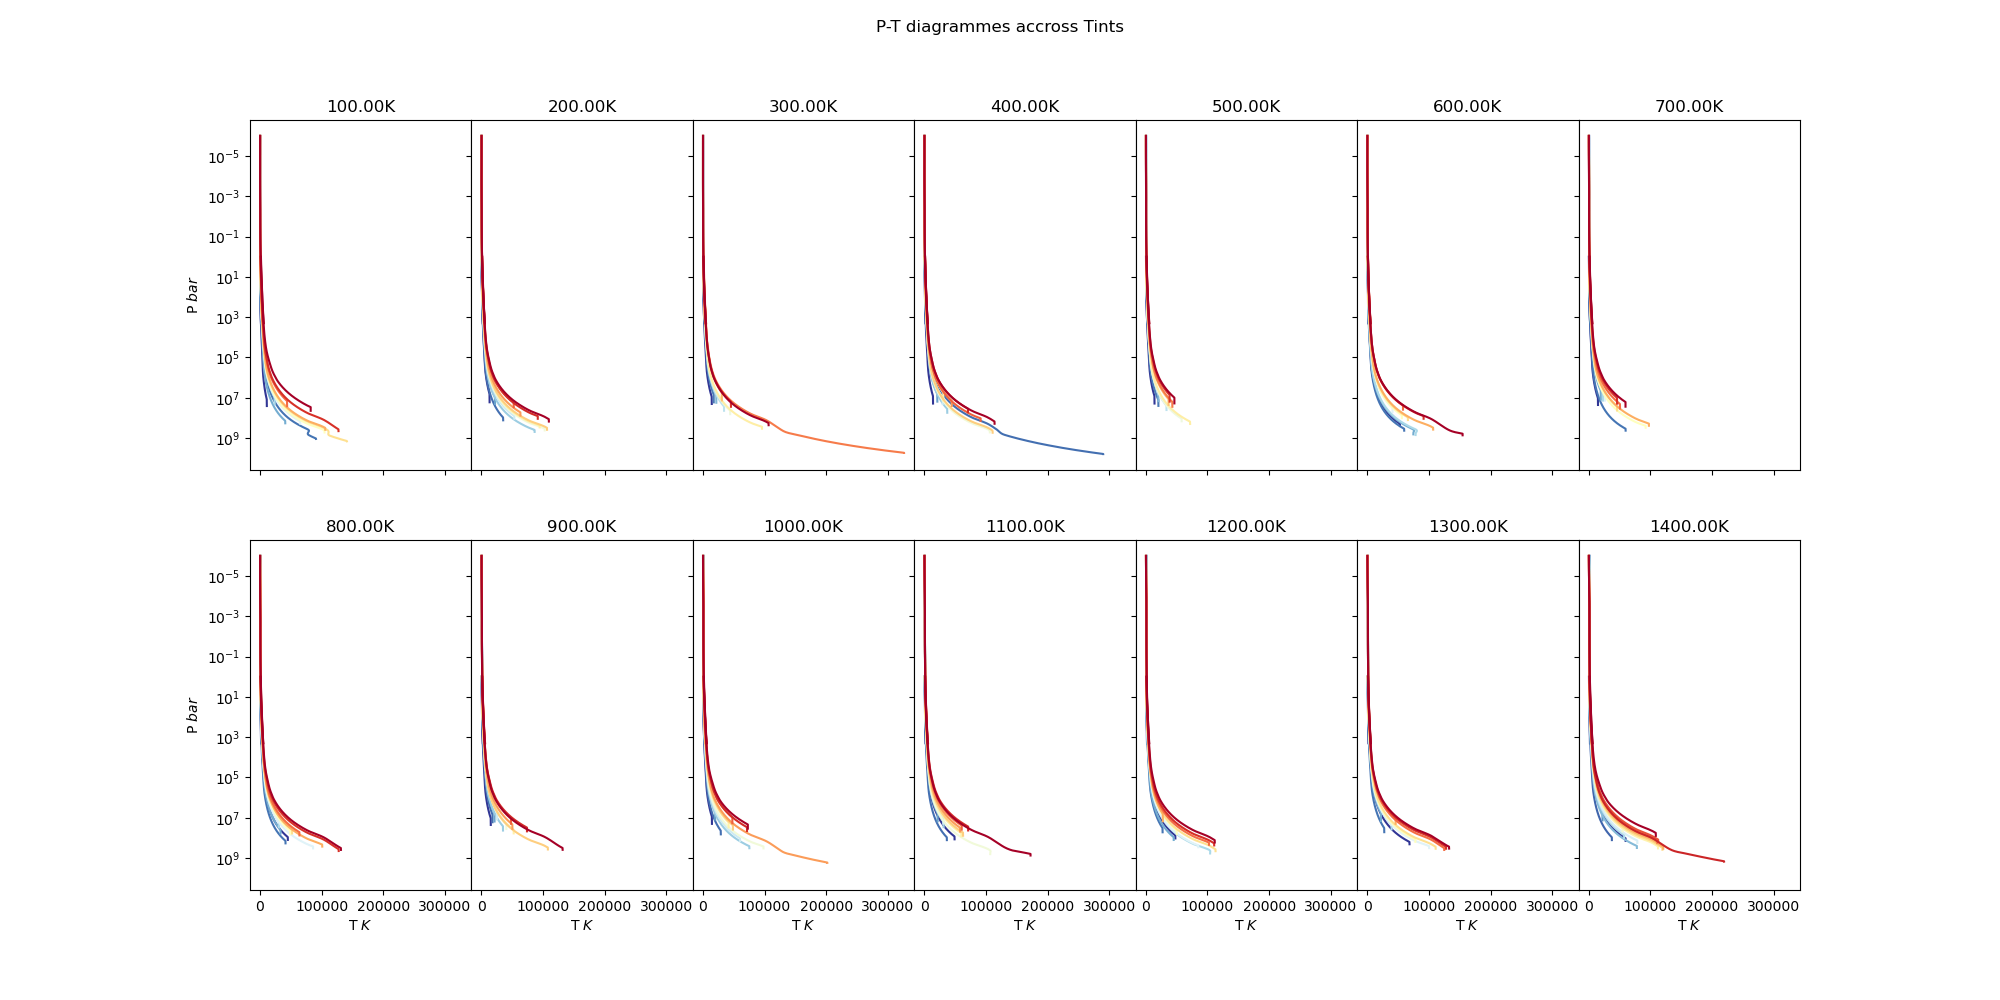
\includegraphics[width=0.48\textwidth]{Images/P_T.png}
    \caption{Pressure temperature profiles each plot at a given irradiation temperature and each profile at a given internal temperature}
    \label{fig:P_T}
\end{figure}

\Cref{fig:M_R_Tint} Shows how the radius is affected by mass, internal temperature and irradiation temperature. We see that higher internal temperatures lead to larger radii. High mass and high internal temperatures lead to a smaller radius than low mass and high temperature. While low temperature and high mass has only a small increase in radius compared to low mass and low internal temperature. It is hard to distinguish differences between different irradiation temperatures from these figures. \par

\begin{figure}
    \centering
    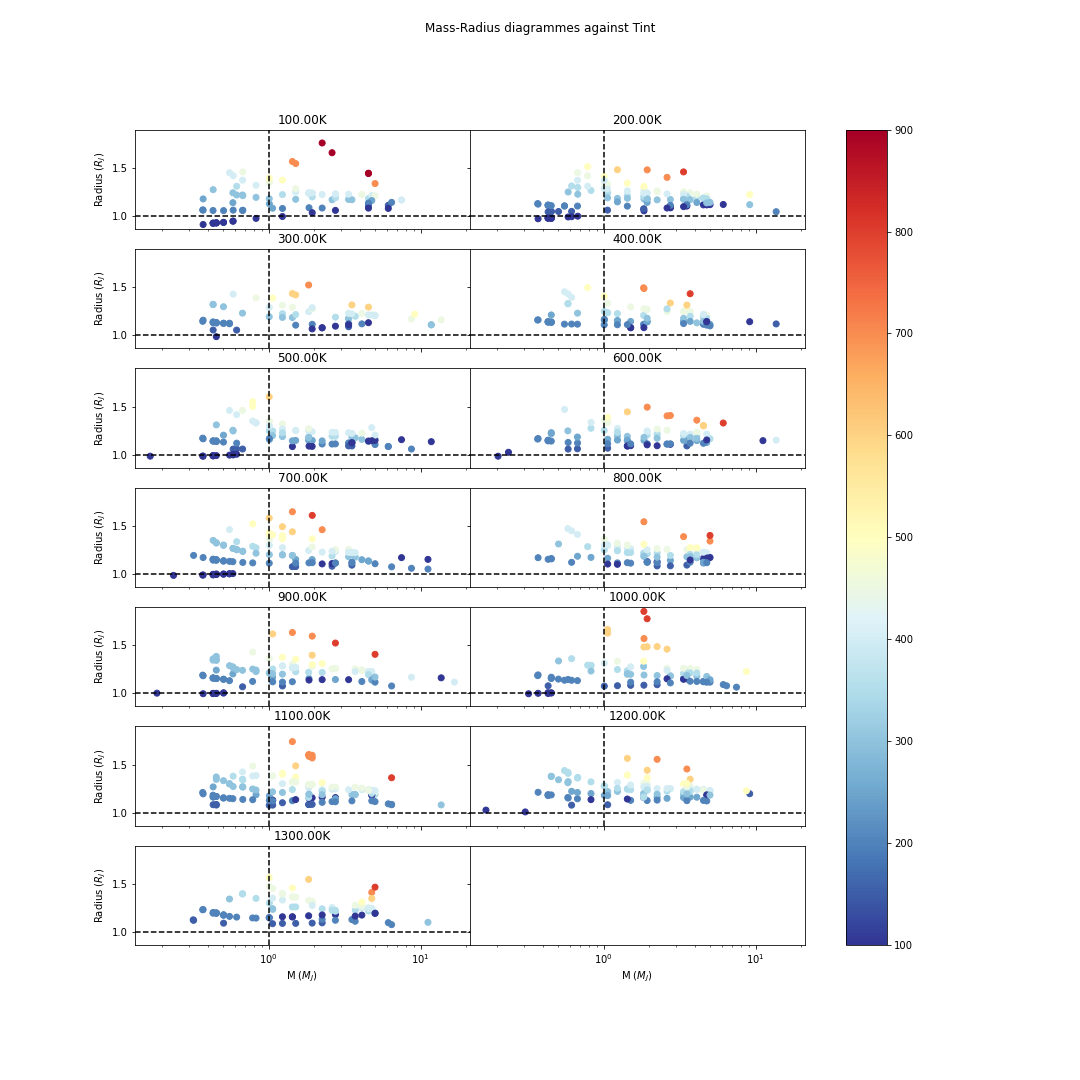
\includegraphics[width=0.48\textwidth]{Images/M_R_Tint.png}
    \caption{Mass Radius plots for different irradiation temperatures, plotted with internal temperature in color axis}
    \label{fig:M_R_Tint}
\end{figure}

\Cref{fig:M_R_Teff} Shows how the radius varies with the effective temperature of the planet. This figure is similar to \cref{fig:M_R_Tint}. The differences are that at high irradiation temperature, the effective temperature is given nearly entirely by the irradiation temperature and we have a degenerate result. \par

\begin{figure}
    \centering
    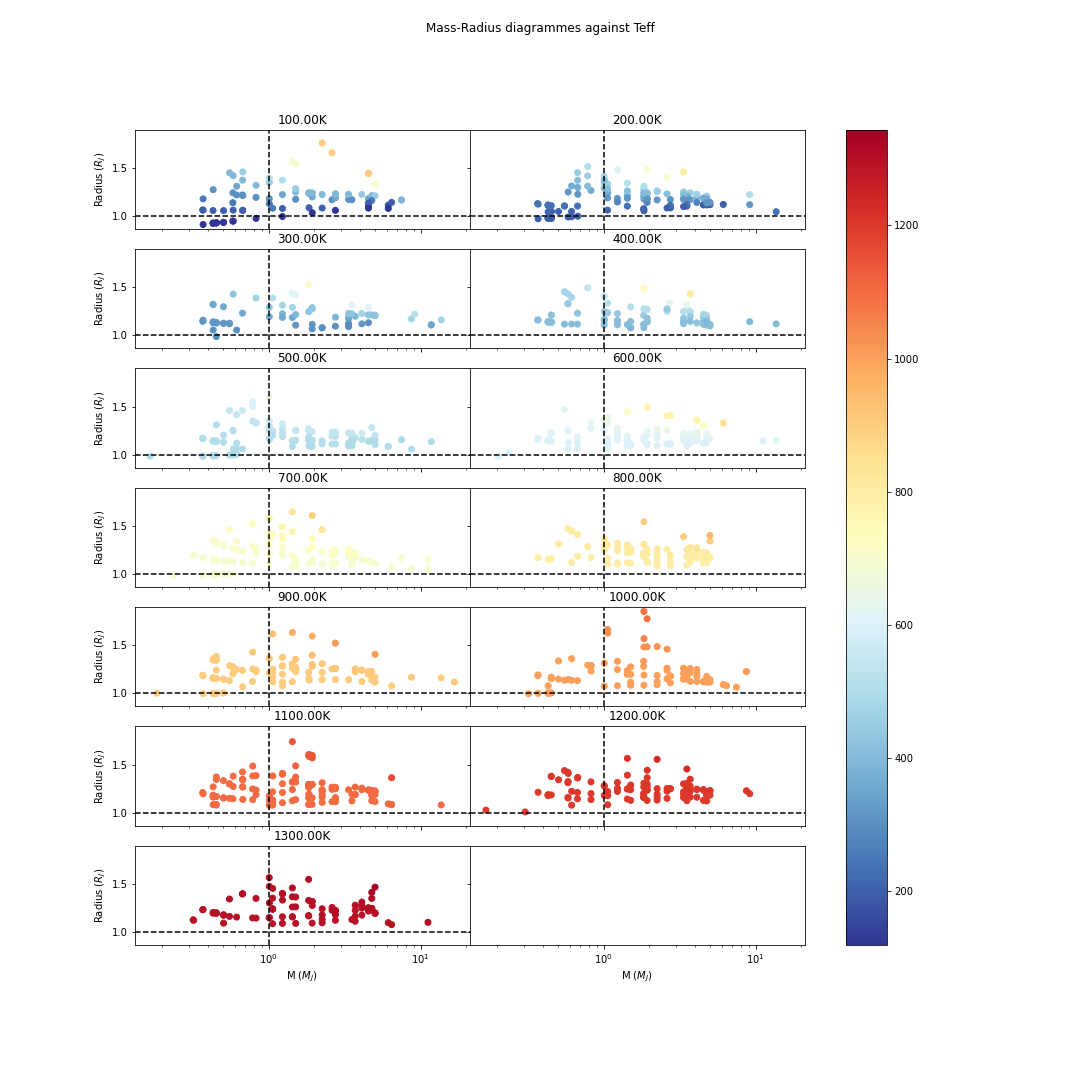
\includegraphics[width=0.48\textwidth]{Images/M_R_Teff.png}
    \caption{Mass Radius plots for different irradiation temperatures, plotted with effective temperature in color axis}
    \label{fig:M_R_Teff}
\end{figure}

\Cref{fig:T_int_R_Tirr} Links the results from \cref{fig:M_R_Tint} so that irradiation temperatures can be compared. We see that in general, higher irradiation temperatures lead to higher radii at a given internal temperature. There seems to be at higher mass a potential inversion of this as internal temperature increases, this however requires further precision to confirm. \par

\begin{figure}
    \centering
    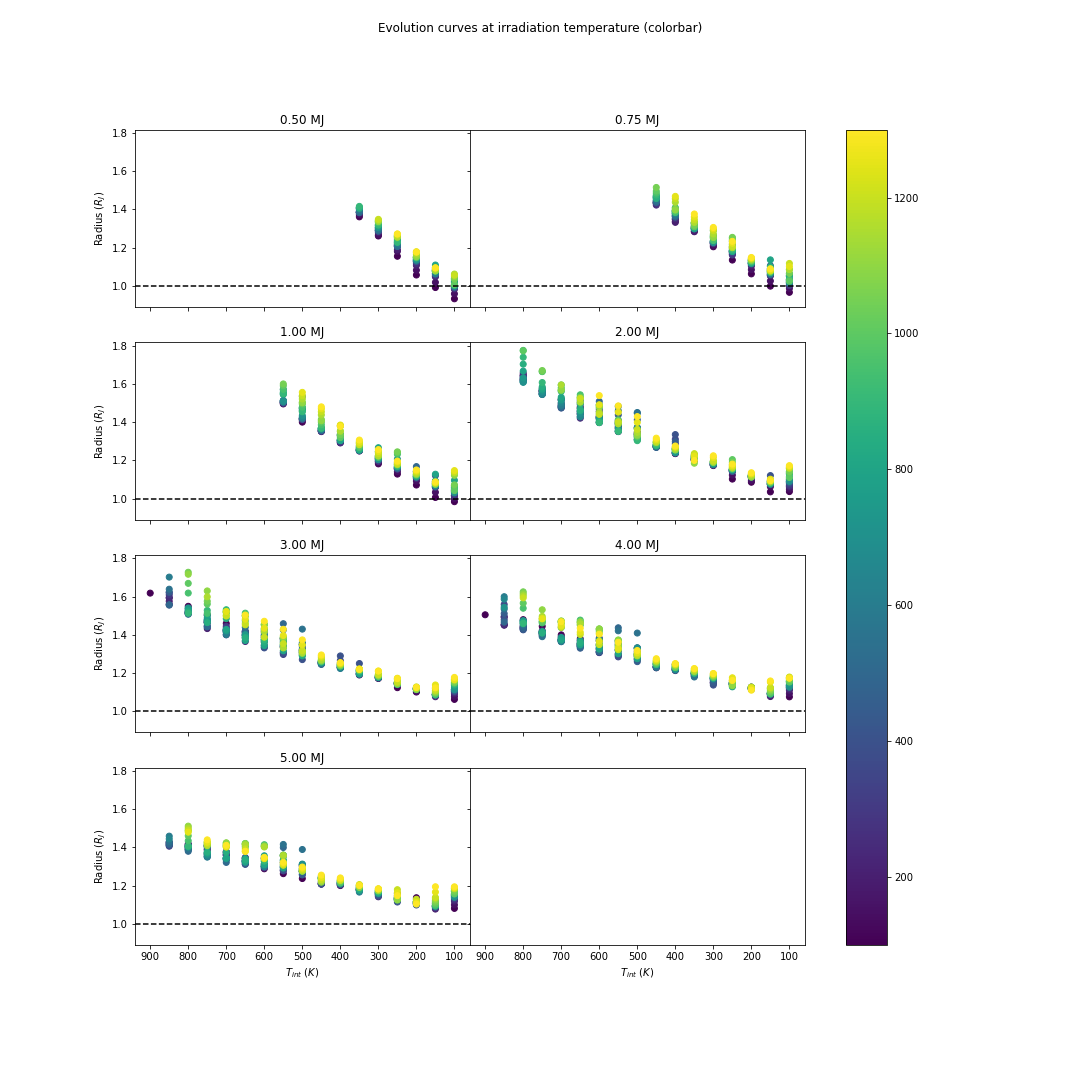
\includegraphics[width=0.48\textwidth]{Images/T_int_R_Tirr.png}
    \caption{Radius as a function of internal temperature for various planetary masses, plotted with irradiation temperatures in color axis}
    \label{fig:T_int_R_Tirr}
\end{figure}

\Cref{fig:T_eff_R_Tirr} is similar to \cref{fig:T_int_R_Tirr}, however we use the effective temperature instead of the internal temperature. This plot is a direct consequence of \cref{fig:M_R_Teff} where we see that for high irradiation temperatures, the effective temperature is equivalent to the irradiation temperature. \par

\begin{figure}
    \centering
    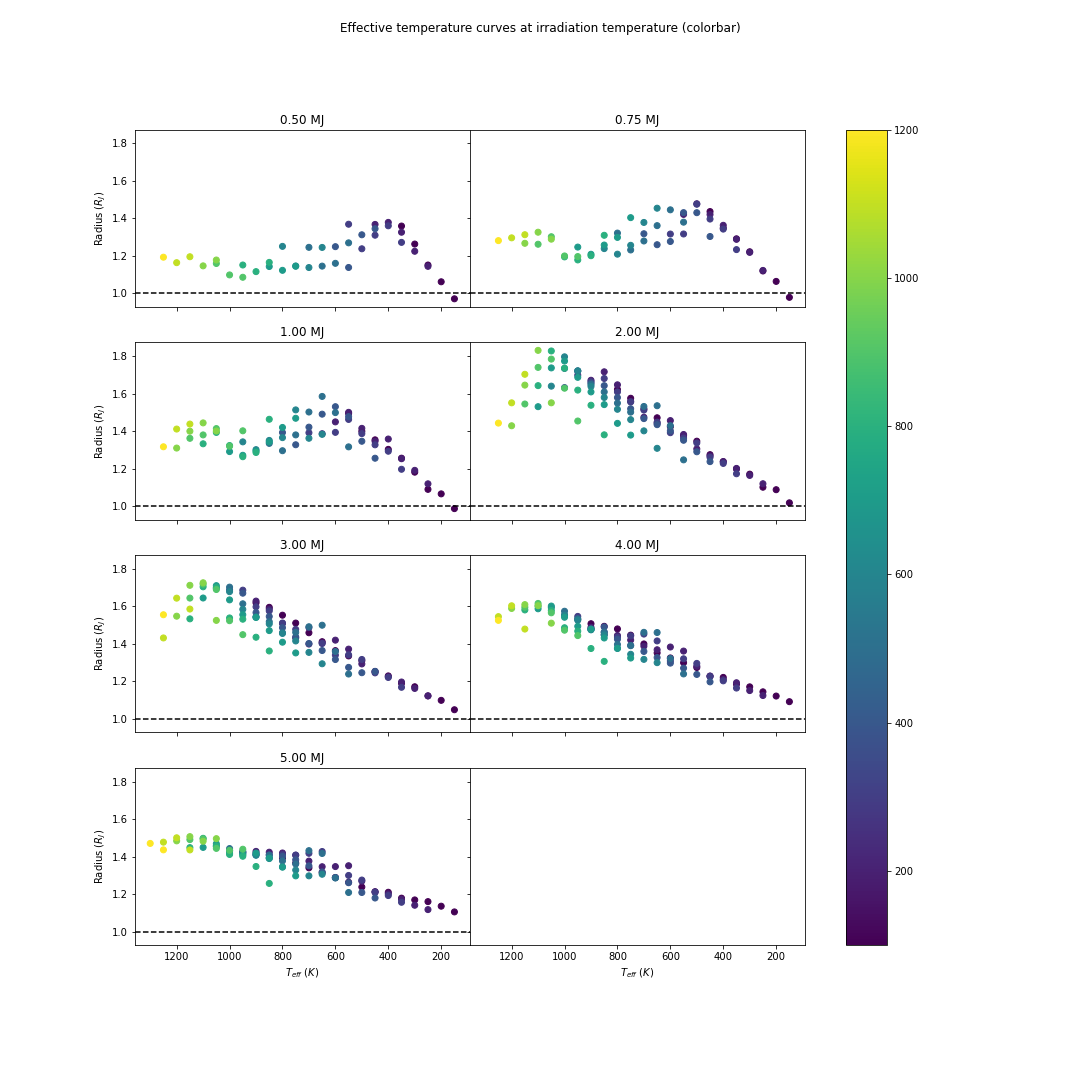
\includegraphics[width=0.48\textwidth]{Images/T_eff_R_Tirr.png}
    \caption{Radius as a function of effective temperature for various planetary masses, plotted with irradiation temperatures in color axis}
    \label{fig:T_eff_R_Tirr}
\end{figure}

\Cref{fig:SR} Shows how the spectral radiosity varies with internal temperature (color gradient) and irradiation temperature. We see that as temperature increases (internal and irradiation) individual spectral features at different wavelengths gradually fade away. \par

\begin{figure}
    \centering
    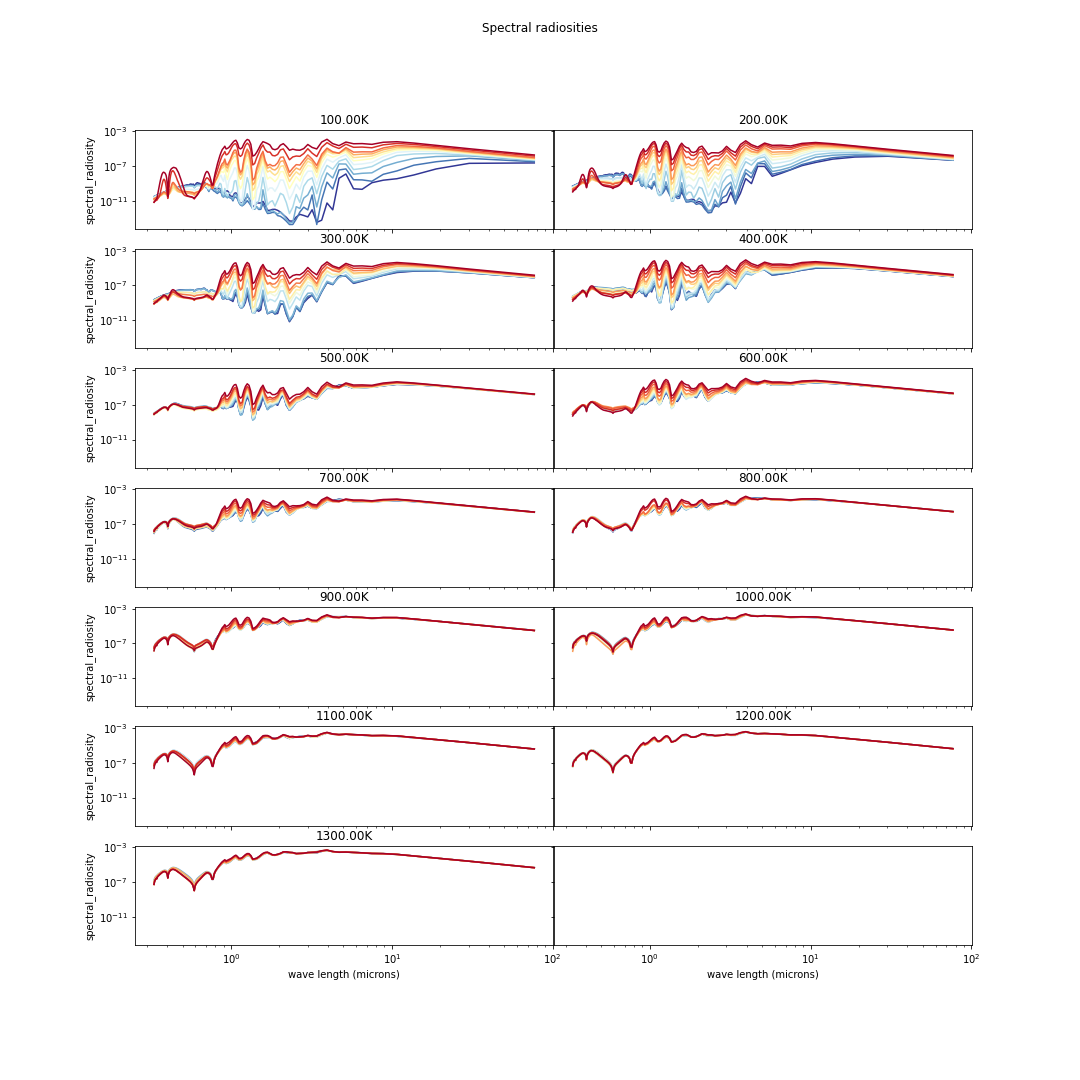
\includegraphics[width=0.48\textwidth]{Images/spectral_radiosity.png}
    \caption{Spectral radiosities for various Irradiation temperatures and internal temperatures (color gradient)}
    \label{fig:SR}
\end{figure}
\section{Litterature comparaison}
% Delete the text and write your Discussion here:
%------------------------------------

In order to estimate the veracity of the combined model presented, we propose to compare where possible to published evolution grids from the literature. The Sonora grid published in 2021\parencite{marley_sonora_2021} uses a cloudless atmosphere in chemical equilibrium with an interior model. It covers a compatible domain of planetary masses. The Sonora grid does not consider irradiation and gives radii as a function of effective temperature. As such to compare as accurately as possible, we propose to use the minimal irradiation temperature available (100K) and vary uniquely internal temperature and mass.\par

\begin{figure}
    \centering
    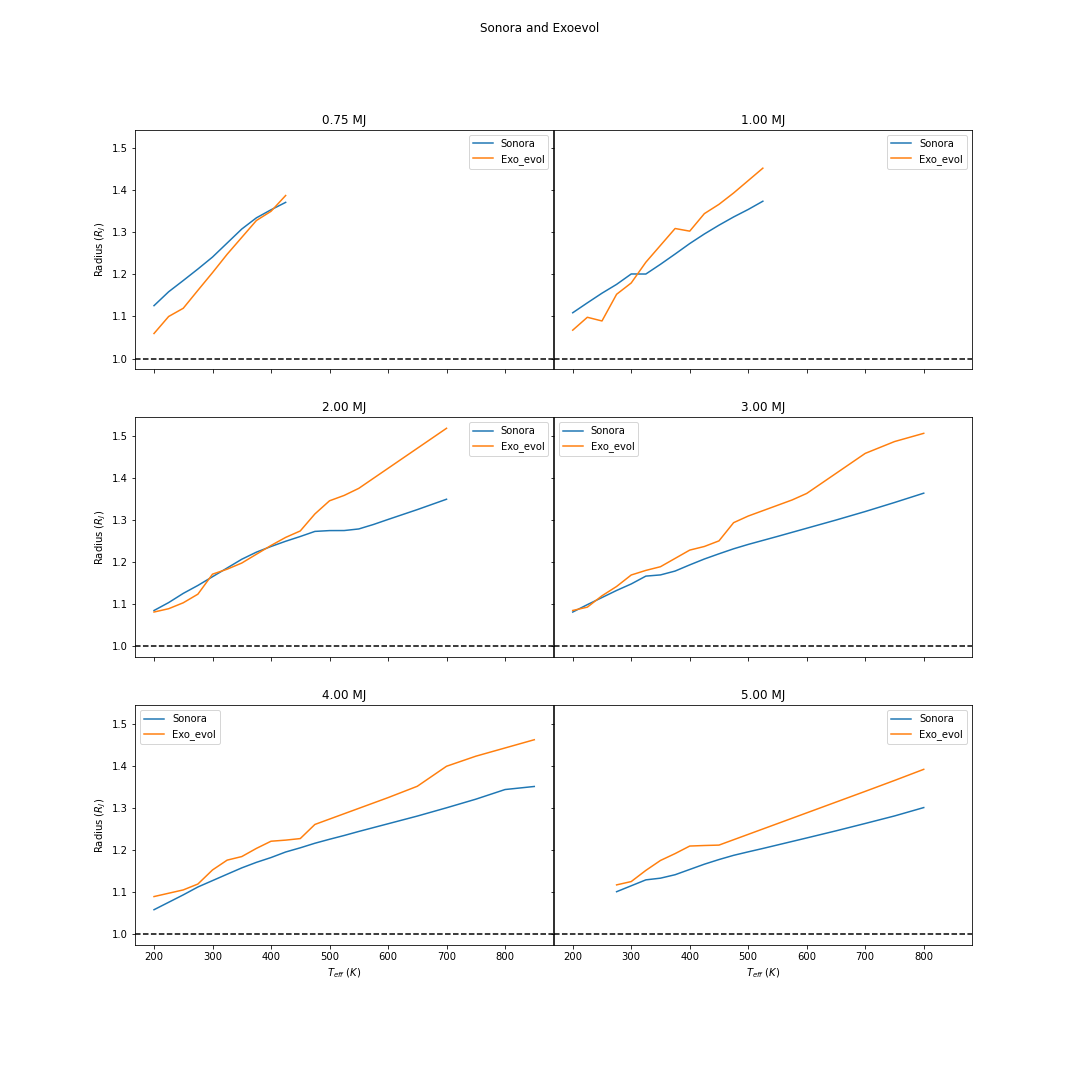
\includegraphics[width=0.48\textwidth]{Images/comp_sonora.png}
    \caption{Sonora and exoevol (exorem+exoris) interpolated to same mass values}
    \label{fig:Son+Exo}
\end{figure}


\begin{figure}
    \centering
    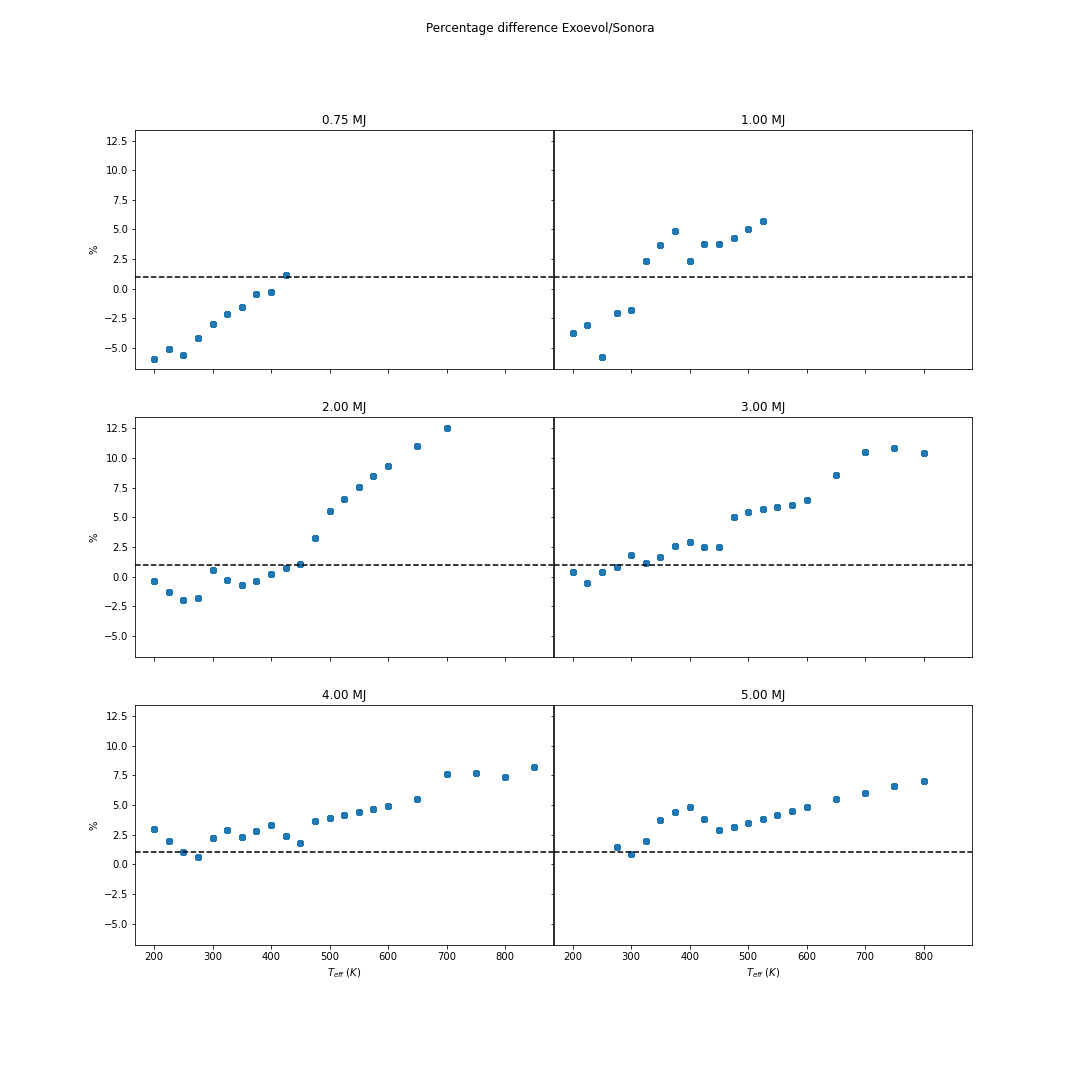
\includegraphics[width=0.48\textwidth]{Images/perc_diff_sonora.png}
    \caption{Percentage difference between Sonora and exoevol (exorem+exoris) at same mass values}
    \label{fig:Son+Exo_perc}
\end{figure}

With \cref{fig:Son+Exo} and \cref{fig:Son+Exo_perc} we see that the difference between the two models remains below around 10\% for the mass and effective temperature range considered. The difference between both models increases with the effective temperature. The differences remain however satisfactory taking into account the at the atmosphere model we use (Exorem) has out of equilibrium chemistry and for the interior model we take into account a core size (10 Earth masses). \par

The Philips et al. model \parencite{phillips_new_2020}  published using the atmo atmosphere model is a useful comparaison as atmo uses an out of equilibrium chemsitry model. Again as irradiation temperature and internal temperatures are not given, we take the non irradiated case (100K irradiation temperature)

\begin{figure}
    \centering
    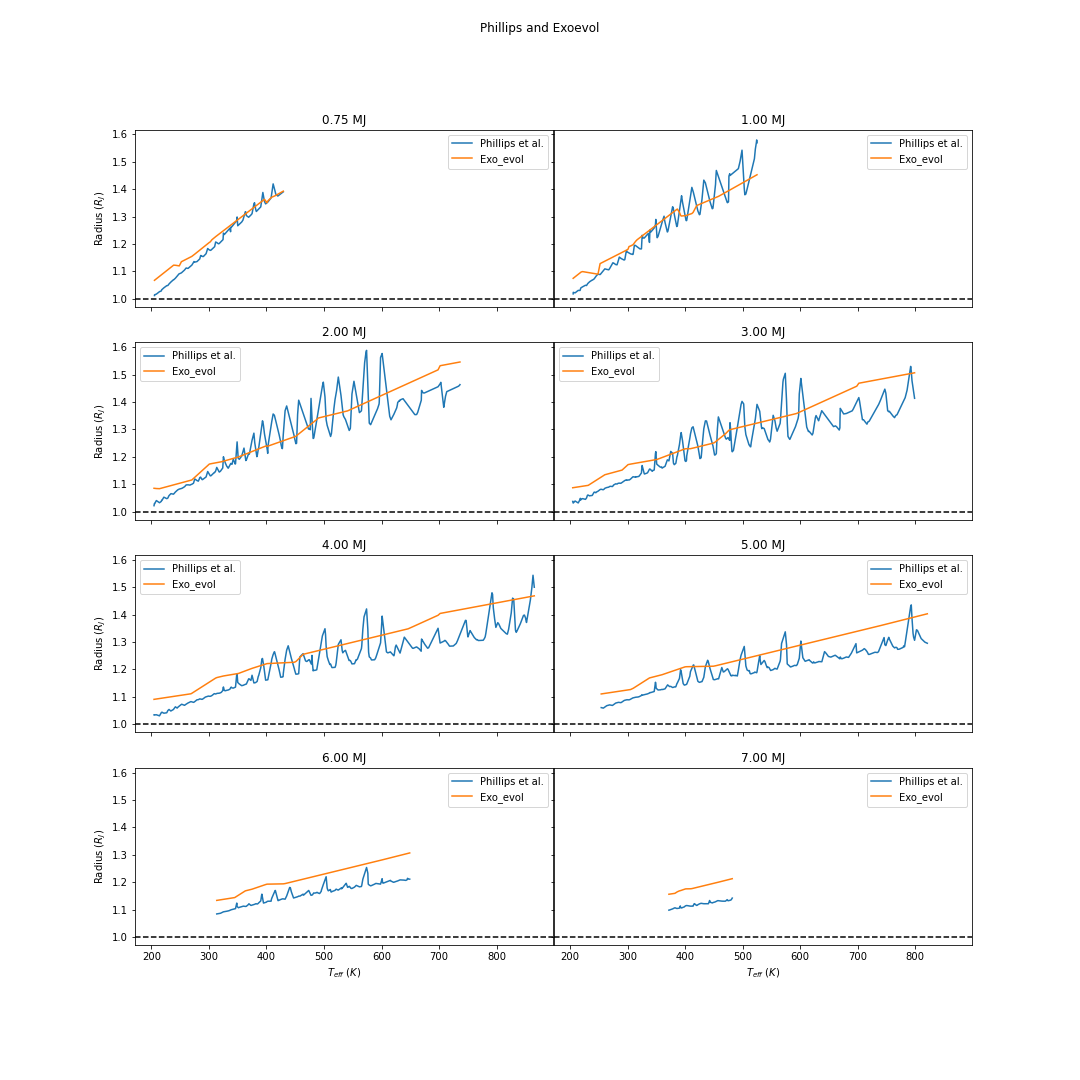
\includegraphics[width=0.48\textwidth]{Images/comp_phillips.png}
    \caption{Phillips et al. and exoevol (exorem+exoris) interpolated to same mass values}
    \label{fig:Phil+Exo}
\end{figure}


\begin{figure}
    \centering
    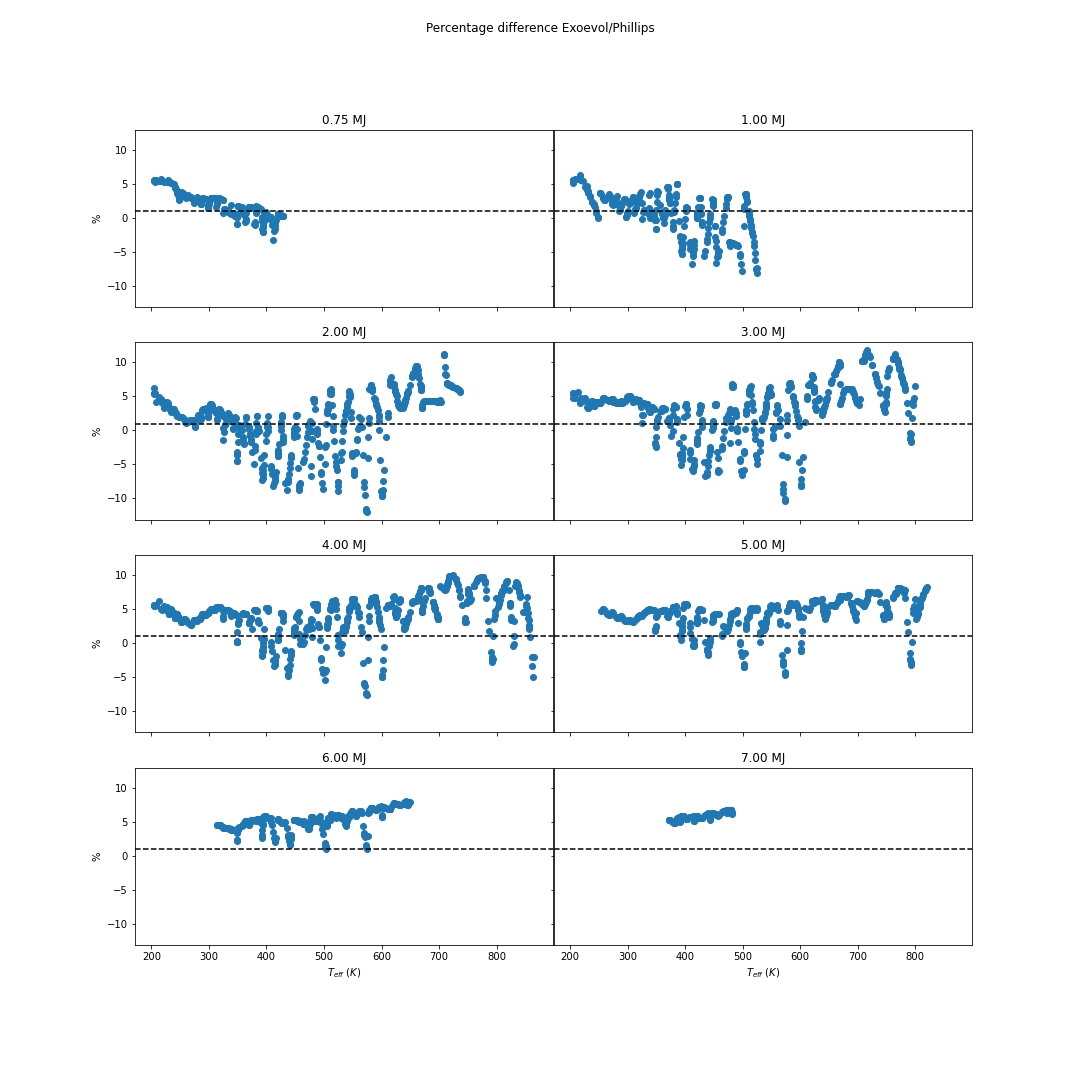
\includegraphics[width=0.48\textwidth]{Images/perc_diff_phillips.png}
    \caption{Percentage difference between Phillips et al. and exoevol (exorem+exoris) at same mass values}
    \label{fig:Phil+Exo_perc}
\end{figure}

(Note oscillations in Phillips et al. data is due to interpolation and requires correcting)

With \cref{fig:Phil+Exo} and \cref{fig:Phil+Exo_perc} we see again that the difference between the two models remains below around 10\% for the mass and effective temperature range considered. The difference between both models is more constant across effective temperature values considered. The choice of the core mass fraction could explain some of the observed differences. A higher core mass than the one considered would lower Exoevol radius closer to that of Philips et al. \par

A comparison transmission spectroscopy is required here.



\section{Application}

We propose to apply the model to the specific example of HD209458b detected via transit in 1999 by Charbonneau et al. \parencite{charbonneau_detection_2000}. HD209458b is a Jupiter like planet with a 0.69 Jupiter mass, with a semi-major axis of 0.04747 AU. It is hence a highly irradiated planet, with an effective temperature of around 1400K. This temperature is currently at the limit of the results previously shown in terms of irradiation temperatures but can still be simulated. We wish to estimate it's internal temperature from it's already estimated Radius of 1.38 Jupiter radii. 

\begin{figure}
    \centering
    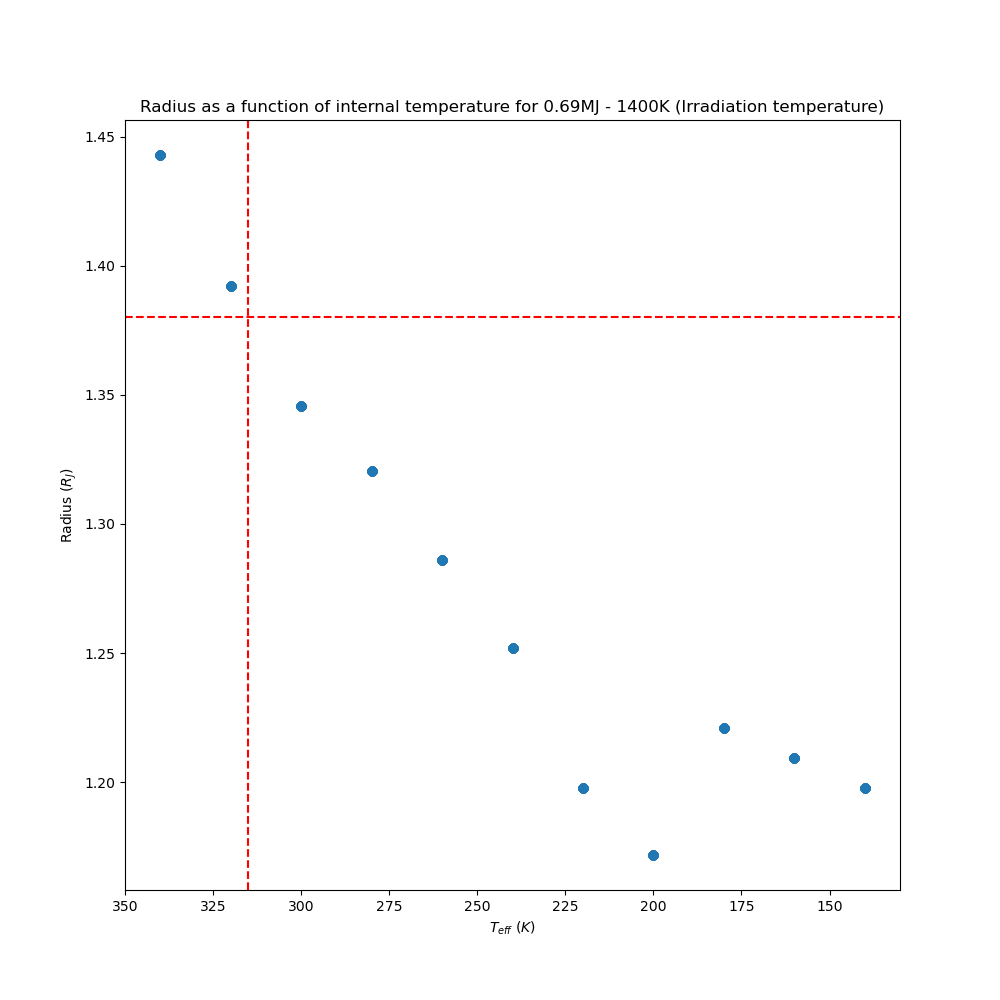
\includegraphics[width=0.48\textwidth]{Images/1400_0.69.png}
    \caption{HD209458b potential evolution curve}
    \label{fig:HD209458b}
\end{figure}

\Cref{fig:HD209458b} indicates that the current internal temperature of HD209458b with the observational parameters is around 320K. We see on this curve that some points appear incorrect, further work is required to understand why some domains of the data are wrong despite the small erreur imposed. However the trend of the whole dataset for the given parameters appears valid. (See annex on interpolation methods)
\section{Conclusion and improvements}
% Delete the text and write your Conclusion here:
%------------------------------------
We see that it is possible to link the Exorem and Exoris model into an evolution model. The obtained results are highly satisfactory when compared to the literature. The application of the model on HD209458b shows that it is possible given observational constraints to estimate planetary parameters. This example also shows further work required. Interpolations to obtain the data for a given planet can only be trustworthy if the dataset is not sparsely populated in the region of interest and the values are given with an error bellow that of the variation in the simulated properties. Work will be required to take into account these uncertainties in order to derive correct error bars on model outputs. Further work is required on the Exoris side of the model, it is common practice to use water instead of Helium to emulate heavier elements, as such this needs to be rapidly implemented before any publication. Adding in cloud cover seems like the next logical step as well as populating the dataset with a range of core values and metallicity. This model goes further than various models currently published due to the out of equilibrium atmosphere chemistry, the use of a planetary core and the capacity to take into account stellar irradiation. In the medium term it seems essential to diversify interior equations of state, most notably if one wishes to derive Neptune like planetary parameters. Further more it would be interesting to compare evolution curves of cloudy models to fingering convection models, this might help differentiate between the two atmospheric dynamics.
%\clearpage                                     % Sometimes you want the rest on separate pages.
\section*{Acknowledgements}
% Delete the text and write Acknowledgements here (not required, can be omitted):
% Comment out ' \section*{Acknowledgements}
% Delete the text and write Acknowledgements here (not required, can be omitted):
% Comment out ' \section*{Acknowledgements}
% Delete the text and write Acknowledgements here (not required, can be omitted):
% Comment out ' \input{Text/Acknowledgements} ' to remove this section.
%------------------------------------
I acknowledge that I have taken a long time to write this report and thank you for your patience. I also acknowledge that there is a lot of work left to do and that I need to hurry up. I acknowledge this is an incorrect use of acknowledgments.
 ' to remove this section.
%------------------------------------
I acknowledge that I have taken a long time to write this report and thank you for your patience. I also acknowledge that there is a lot of work left to do and that I need to hurry up. I acknowledge this is an incorrect use of acknowledgments.
 ' to remove this section.
%------------------------------------
I acknowledge that I have taken a long time to write this report and thank you for your patience. I also acknowledge that there is a lot of work left to do and that I need to hurry up. I acknowledge this is an incorrect use of acknowledgments.
                   % Comment out to exclude the Acknowledgements section

%%%%%%%%%%%%%%%%%%%%%%%%%%%%%%%%%%%%%%%%

% Bibliography
%--------------------
\printbibliography

%\clearpage                                     % Sometimes it is useful to have appendix on separate page.
%\onecolumn                                     % If you want 1 column for appendix.
\appendix
% Delete the text and write Appendix here (not required, can be omitted):
% Comment out ' \appendix
% Delete the text and write Appendix here (not required, can be omitted):
% Comment out ' \appendix
% Delete the text and write Appendix here (not required, can be omitted):
% Comment out ' \input{Text/Appendix} ' to remove this section.
%------------------------------------

\section{Notes on interpolation}

In a 2d space interpolations car be relatively simple, let's consider the following :

\begin{align} 
    (x,y) \in (R,R)
\end{align}

Let us suppose there is some kind of function linking the two, we hence have :

\begin{align} 
    f(x) = y
\end{align}

Should we consider two points of the function $(x_0,y_0)$ and $(x_1,y_1)$ and seek to find the value of a given unknown third point $(x_a,y_a)$ then one would instinctively do a linear interpolation as follows :

\begin{align} 
    \frac{x_1-x_0}{y_1-y_0} (x_a-x_0) + y_0 = y_a
    \label{eq:interp1d}
\end{align}

Should we desire to interpolate at a higher order, we can use the Lagrange set of polynomes as follows:

\begin{align} 
    y(x) = \sum_{j=0}^{k} y_j c_j(x)
        c_j(x) = \ell_j(x,x_0,x_1,\ldots,x_k) = \nonumber \\
        \prod_{\begin{smallmatrix}0\le m\le k\\ m\neq j\end{smallmatrix}} \frac{x-x_m}{x_j-x_m} = \nonumber \\
        \frac{(x-x_0)}{(x_j-x_0)} \cdots \frac{(x-x_{j-1})}{(x_j-x_{j-1})} \frac{(x-x_{j+1})}{(x_j-x_{j+1})} \cdots \frac{(x-x_k)}{(x_j-x_k)}
\end{align}

For a polynome of order $k$ we require $k+1$ node points, this is an important point to keep in mind when constructing a grid to subsequently interpolate. Interpolation residuals will not be detailed here. As all that is explicated here can be found in any math book, the more curious reader can quite easily find further details.

Another way of of seeing \cref{eq:interp1d} is as evaluating the barycenter along a line. where the term $x_a-x_0$ represents the displacement from $x_0$ to $x$. Generalised, it is possible to write the higher order polynomial approximation in terms of the displacement from a given point.

\begin{align} 
    L(x) = \ell(x) \sum_{j=0}^k \frac{w_j}{x-x_j}y_j
\end{align}

In practice this means that we consider a set of values $f(x_j)=y_j$ close to the desired point and interpolate the point by weighting the $f(x_j)$ values by the distance $x-x_j$ to that given point.

That which is given here is valid in a two dimensional space but for parts of the work, it is required to interpolate in higher dimension. To quote "Méthode numériques appliquées" by Jean-Philippe Grivet \parencite{Methodes_numerique_appliques} : "The algorithms described above can be generalized in a more or less laborious way to two or more dimensions." This has been one of the challenges to overcome in this work. Indeed for perfectly regular grids, it is possible to derive semi-analytical equations using methods such as bi-cubic interpolations, however here our grids will, through iterative steps, no longer be regular. We propose to overcome this problem to use a barycentric interpolation using a Delauney triangulation. In terms of the barycentric interpolation the method is the same as the logic presented above. We weight the distance between nodes by the distance to the desired point and that for a group of points that surround our point of interest. However the surrounding of a point in higher dimension is a non negligible task. A Delaunay triangulation in a two dimensional space is a triangulation for which no point of the grid is in the circumcircle of another triangle, where a triangle is defined by three points of the grid. If one draws this condition out one will notice that this splits a space into triangles with no points inside those triangles. For a higher dimensional space, the circumcircle becomes a circum-hypersphere. The mathematical details will be left to the most curious readers.\par

In practice, the methods presented were not coded but imported from the python Scipy library. However it is essential when using interpolations to know what is being done. Interpolations if used incorrectly can lead to erroneous results which can appear correct. For this reason we do not explicit extrapolations as any desired data points outside of the grid are deemed only accessible if the grid is extended by running the underlying models. This poses a new challenge, how to correctly extend the grid in order to subsequently perform interpolations. If computational time is plenteous than a random grid search can be completed, otherwise an extrapolation can be carried out with the objective of running the underlying models at the extrapolation point. This is yet to be correctly done.

\section{Notes on degeneracy}

\Cref{fig:Degen} gives an example of partial ternary degeneracy plot generated with Exoris where we see how the radius for a planet at a given mass varies depending on its mass fraction composition. Where the color is the same, we have a degeneracy. We see that it is possible to have the same radius for various mass fractions of hydrogen, helium and core. This plot explicates the need to link interior models with atmosphere models. Indeed the hydrogen and helium mass fractions here are ultimately fixed by the atmosphere model. The core is therefore left as a free parameter, however if the radius of a planet is known it is possible to remove all degeneracy presented here. The more critical reader could think that fundamentally this is just pushing the problem up into the atmosphere, this is true, however as photons escape from radiative zones in the atmosphere, it is theoretically possible with a perfect observation to resolve this internal structure as presented here. However internal structures can be more complex than this diagram indicates. The core can have rock and ice composition, with distinct fractions of both. We can also imagine for Neptune like planets layers of water/ice in the envelope, in which case the degeneracy plot becomes more complicated and further work is required in order to understand what remains degenerate after model linkage.

\begin{figure}
    \centering
    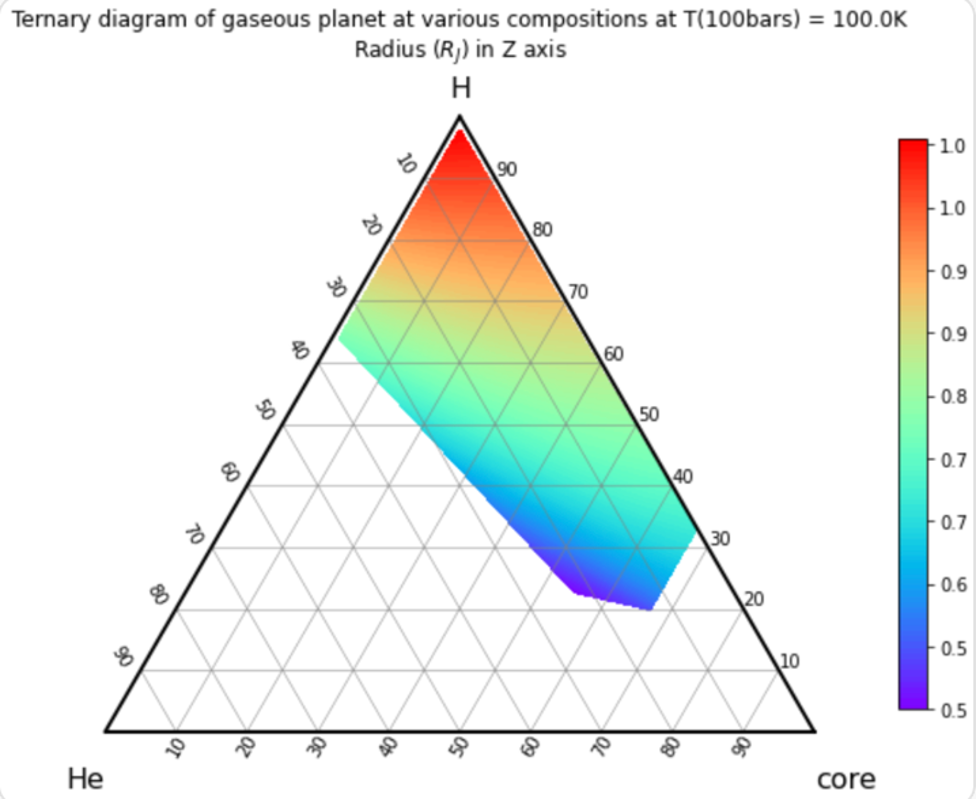
\includegraphics[width=0.48\textwidth]{Images/degeneracies.png}
    \caption{Degeneracy plot (ternary plot), representing radius ($R_J$) at various, hydrogen, helium and core mass fractions}
    \label{fig:Degen}
\end{figure}

\section{Notes on exorem model selection}

As stated in the model description, exorem can in certain conditions struggle to converge. This happens generally in zones of the grid where the irradiation temperature is low and internal temperature high. Exorem can not balance the two stream flux model and balance the temperature at the bottom and top of the atmosphere. To deal with this, we help Exorem converge either by relying on T. Guillot (2010) \parencite{guillot_radiative_2010} non grey analytical model to provide initial pressure temperature profiles to guide exorem, these do not take into account irradiation. We can also re-inject profiles from the grid into Exorem, to accomplish this we find the closest profile to the given input parameters. However often this does not suffice and we still have non-converged profiles. It would be taking a risk to leave these profiles in the grid especially taking into account that for the moment we do not use any smoothing in the interpolation methods considered above. As such we chose to remove these profiles. Through trial and error it was shown that a systematic code to identify bad profiles was inefficient. As such a simple tree based model was used to identify such profiles. To do this a LGBM classifier was trained. LGBM classifiers are gradient boosted tree based learning algorithms that have low memory usage and are more efficient than most other classifiers such as random forests. They use leaf wise tree growth which increases efficiency. The disadvantage of such classifiers are that they are very sensitive to over-fitting and require relatively large data-sets. The model was trained using the top atmosphere flux ratio, bottom atmosphere flux ratio, effective temperature ratio, internal temperature and irradiation temperature. The more data science orientated reader might be concerned when seeing that dimensional data was used as a feature. We allowed ourselves to do this as the internal temperature and irradiation temperature are bounded by the grid limits, rigorously one should divide these values by their maximum value on the grid. The results obtained were an accurate categorisation of 98\% of profiles, with an equal split percentage wise between false positives and false negatives. 

\section{Notes on entropy of mixes}

As shown in \parencite{chabrier_new_2019}, the expression for a given extensive quantity $W$ at a given $(T,P)$ for a mixture is given by :

\begin{align} 
    W(T,P) = \sum_{i} X_{i} W_{i}(T,P)
    \label{eq:extensive_qty}
\end{align}

With :

\begin{align} 
    X_{i} = \frac{M_i}{\sum_{i}M_{i}}
    \label{eq:mass_fraction}
\end{align}

Subsequently we can express the entropy of a mix of $He/H/H_2O$ as follows :

\begin{align} 
    S = \sum_{i} X_{i} S_{i}(T,P) + S_{mix}(T,P)
    \label{eq:entropy_mix1}
\end{align}

\begin{align} 
    S = X_{H} S_{H}(T,P) + X_{He} S_{He}(T,P) \nonumber \\ 
    + X_{H_2O} S_{H_2O}(T,P) + S_{mix}(T,P)
    \label{eq:entropy_mix2}
\end{align}

With here $S_{mix}(T,P)$ the ideal mixing term that we will better define subsequently. But we shall consider equal to zero.

We need to substitute the expressions for the mass fractions.  ' to remove this section.
%------------------------------------

\section{Notes on interpolation}

In a 2d space interpolations car be relatively simple, let's consider the following :

\begin{align} 
    (x,y) \in (R,R)
\end{align}

Let us suppose there is some kind of function linking the two, we hence have :

\begin{align} 
    f(x) = y
\end{align}

Should we consider two points of the function $(x_0,y_0)$ and $(x_1,y_1)$ and seek to find the value of a given unknown third point $(x_a,y_a)$ then one would instinctively do a linear interpolation as follows :

\begin{align} 
    \frac{x_1-x_0}{y_1-y_0} (x_a-x_0) + y_0 = y_a
    \label{eq:interp1d}
\end{align}

Should we desire to interpolate at a higher order, we can use the Lagrange set of polynomes as follows:

\begin{align} 
    y(x) = \sum_{j=0}^{k} y_j c_j(x)
        c_j(x) = \ell_j(x,x_0,x_1,\ldots,x_k) = \nonumber \\
        \prod_{\begin{smallmatrix}0\le m\le k\\ m\neq j\end{smallmatrix}} \frac{x-x_m}{x_j-x_m} = \nonumber \\
        \frac{(x-x_0)}{(x_j-x_0)} \cdots \frac{(x-x_{j-1})}{(x_j-x_{j-1})} \frac{(x-x_{j+1})}{(x_j-x_{j+1})} \cdots \frac{(x-x_k)}{(x_j-x_k)}
\end{align}

For a polynome of order $k$ we require $k+1$ node points, this is an important point to keep in mind when constructing a grid to subsequently interpolate. Interpolation residuals will not be detailed here. As all that is explicated here can be found in any math book, the more curious reader can quite easily find further details.

Another way of of seeing \cref{eq:interp1d} is as evaluating the barycenter along a line. where the term $x_a-x_0$ represents the displacement from $x_0$ to $x$. Generalised, it is possible to write the higher order polynomial approximation in terms of the displacement from a given point.

\begin{align} 
    L(x) = \ell(x) \sum_{j=0}^k \frac{w_j}{x-x_j}y_j
\end{align}

In practice this means that we consider a set of values $f(x_j)=y_j$ close to the desired point and interpolate the point by weighting the $f(x_j)$ values by the distance $x-x_j$ to that given point.

That which is given here is valid in a two dimensional space but for parts of the work, it is required to interpolate in higher dimension. To quote "Méthode numériques appliquées" by Jean-Philippe Grivet \parencite{Methodes_numerique_appliques} : "The algorithms described above can be generalized in a more or less laborious way to two or more dimensions." This has been one of the challenges to overcome in this work. Indeed for perfectly regular grids, it is possible to derive semi-analytical equations using methods such as bi-cubic interpolations, however here our grids will, through iterative steps, no longer be regular. We propose to overcome this problem to use a barycentric interpolation using a Delauney triangulation. In terms of the barycentric interpolation the method is the same as the logic presented above. We weight the distance between nodes by the distance to the desired point and that for a group of points that surround our point of interest. However the surrounding of a point in higher dimension is a non negligible task. A Delaunay triangulation in a two dimensional space is a triangulation for which no point of the grid is in the circumcircle of another triangle, where a triangle is defined by three points of the grid. If one draws this condition out one will notice that this splits a space into triangles with no points inside those triangles. For a higher dimensional space, the circumcircle becomes a circum-hypersphere. The mathematical details will be left to the most curious readers.\par

In practice, the methods presented were not coded but imported from the python Scipy library. However it is essential when using interpolations to know what is being done. Interpolations if used incorrectly can lead to erroneous results which can appear correct. For this reason we do not explicit extrapolations as any desired data points outside of the grid are deemed only accessible if the grid is extended by running the underlying models. This poses a new challenge, how to correctly extend the grid in order to subsequently perform interpolations. If computational time is plenteous than a random grid search can be completed, otherwise an extrapolation can be carried out with the objective of running the underlying models at the extrapolation point. This is yet to be correctly done.

\section{Notes on degeneracy}

\Cref{fig:Degen} gives an example of partial ternary degeneracy plot generated with Exoris where we see how the radius for a planet at a given mass varies depending on its mass fraction composition. Where the color is the same, we have a degeneracy. We see that it is possible to have the same radius for various mass fractions of hydrogen, helium and core. This plot explicates the need to link interior models with atmosphere models. Indeed the hydrogen and helium mass fractions here are ultimately fixed by the atmosphere model. The core is therefore left as a free parameter, however if the radius of a planet is known it is possible to remove all degeneracy presented here. The more critical reader could think that fundamentally this is just pushing the problem up into the atmosphere, this is true, however as photons escape from radiative zones in the atmosphere, it is theoretically possible with a perfect observation to resolve this internal structure as presented here. However internal structures can be more complex than this diagram indicates. The core can have rock and ice composition, with distinct fractions of both. We can also imagine for Neptune like planets layers of water/ice in the envelope, in which case the degeneracy plot becomes more complicated and further work is required in order to understand what remains degenerate after model linkage.

\begin{figure}
    \centering
    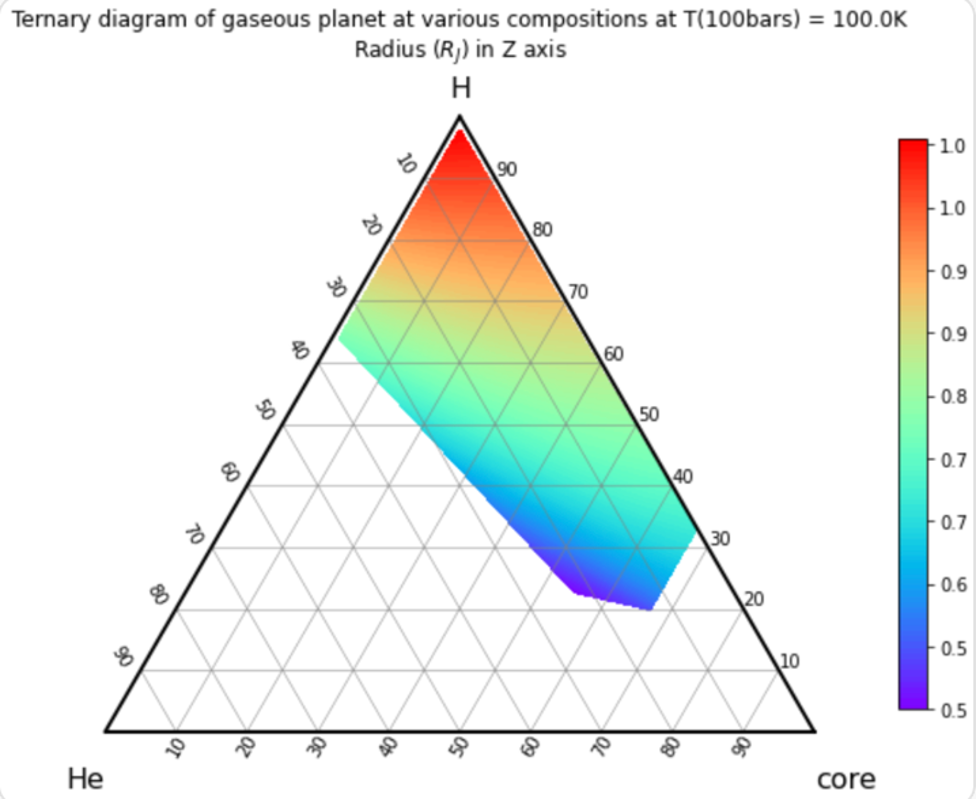
\includegraphics[width=0.48\textwidth]{Images/degeneracies.png}
    \caption{Degeneracy plot (ternary plot), representing radius ($R_J$) at various, hydrogen, helium and core mass fractions}
    \label{fig:Degen}
\end{figure}

\section{Notes on exorem model selection}

As stated in the model description, exorem can in certain conditions struggle to converge. This happens generally in zones of the grid where the irradiation temperature is low and internal temperature high. Exorem can not balance the two stream flux model and balance the temperature at the bottom and top of the atmosphere. To deal with this, we help Exorem converge either by relying on T. Guillot (2010) \parencite{guillot_radiative_2010} non grey analytical model to provide initial pressure temperature profiles to guide exorem, these do not take into account irradiation. We can also re-inject profiles from the grid into Exorem, to accomplish this we find the closest profile to the given input parameters. However often this does not suffice and we still have non-converged profiles. It would be taking a risk to leave these profiles in the grid especially taking into account that for the moment we do not use any smoothing in the interpolation methods considered above. As such we chose to remove these profiles. Through trial and error it was shown that a systematic code to identify bad profiles was inefficient. As such a simple tree based model was used to identify such profiles. To do this a LGBM classifier was trained. LGBM classifiers are gradient boosted tree based learning algorithms that have low memory usage and are more efficient than most other classifiers such as random forests. They use leaf wise tree growth which increases efficiency. The disadvantage of such classifiers are that they are very sensitive to over-fitting and require relatively large data-sets. The model was trained using the top atmosphere flux ratio, bottom atmosphere flux ratio, effective temperature ratio, internal temperature and irradiation temperature. The more data science orientated reader might be concerned when seeing that dimensional data was used as a feature. We allowed ourselves to do this as the internal temperature and irradiation temperature are bounded by the grid limits, rigorously one should divide these values by their maximum value on the grid. The results obtained were an accurate categorisation of 98\% of profiles, with an equal split percentage wise between false positives and false negatives. 

\section{Notes on entropy of mixes}

As shown in \parencite{chabrier_new_2019}, the expression for a given extensive quantity $W$ at a given $(T,P)$ for a mixture is given by :

\begin{align} 
    W(T,P) = \sum_{i} X_{i} W_{i}(T,P)
    \label{eq:extensive_qty}
\end{align}

With :

\begin{align} 
    X_{i} = \frac{M_i}{\sum_{i}M_{i}}
    \label{eq:mass_fraction}
\end{align}

Subsequently we can express the entropy of a mix of $He/H/H_2O$ as follows :

\begin{align} 
    S = \sum_{i} X_{i} S_{i}(T,P) + S_{mix}(T,P)
    \label{eq:entropy_mix1}
\end{align}

\begin{align} 
    S = X_{H} S_{H}(T,P) + X_{He} S_{He}(T,P) \nonumber \\ 
    + X_{H_2O} S_{H_2O}(T,P) + S_{mix}(T,P)
    \label{eq:entropy_mix2}
\end{align}

With here $S_{mix}(T,P)$ the ideal mixing term that we will better define subsequently. But we shall consider equal to zero.

We need to substitute the expressions for the mass fractions.  ' to remove this section.
%------------------------------------

\section{Notes on interpolation}

In a 2d space interpolations car be relatively simple, let's consider the following :

\begin{align} 
    (x,y) \in (R,R)
\end{align}

Let us suppose there is some kind of function linking the two, we hence have :

\begin{align} 
    f(x) = y
\end{align}

Should we consider two points of the function $(x_0,y_0)$ and $(x_1,y_1)$ and seek to find the value of a given unknown third point $(x_a,y_a)$ then one would instinctively do a linear interpolation as follows :

\begin{align} 
    \frac{x_1-x_0}{y_1-y_0} (x_a-x_0) + y_0 = y_a
    \label{eq:interp1d}
\end{align}

Should we desire to interpolate at a higher order, we can use the Lagrange set of polynomes as follows:

\begin{align} 
    y(x) = \sum_{j=0}^{k} y_j c_j(x)
        c_j(x) = \ell_j(x,x_0,x_1,\ldots,x_k) = \nonumber \\
        \prod_{\begin{smallmatrix}0\le m\le k\\ m\neq j\end{smallmatrix}} \frac{x-x_m}{x_j-x_m} = \nonumber \\
        \frac{(x-x_0)}{(x_j-x_0)} \cdots \frac{(x-x_{j-1})}{(x_j-x_{j-1})} \frac{(x-x_{j+1})}{(x_j-x_{j+1})} \cdots \frac{(x-x_k)}{(x_j-x_k)}
\end{align}

For a polynome of order $k$ we require $k+1$ node points, this is an important point to keep in mind when constructing a grid to subsequently interpolate. Interpolation residuals will not be detailed here. As all that is explicated here can be found in any math book, the more curious reader can quite easily find further details.

Another way of of seeing \cref{eq:interp1d} is as evaluating the barycenter along a line. where the term $x_a-x_0$ represents the displacement from $x_0$ to $x$. Generalised, it is possible to write the higher order polynomial approximation in terms of the displacement from a given point.

\begin{align} 
    L(x) = \ell(x) \sum_{j=0}^k \frac{w_j}{x-x_j}y_j
\end{align}

In practice this means that we consider a set of values $f(x_j)=y_j$ close to the desired point and interpolate the point by weighting the $f(x_j)$ values by the distance $x-x_j$ to that given point.

That which is given here is valid in a two dimensional space but for parts of the work, it is required to interpolate in higher dimension. To quote "Méthode numériques appliquées" by Jean-Philippe Grivet \parencite{Methodes_numerique_appliques} : "The algorithms described above can be generalized in a more or less laborious way to two or more dimensions." This has been one of the challenges to overcome in this work. Indeed for perfectly regular grids, it is possible to derive semi-analytical equations using methods such as bi-cubic interpolations, however here our grids will, through iterative steps, no longer be regular. We propose to overcome this problem to use a barycentric interpolation using a Delauney triangulation. In terms of the barycentric interpolation the method is the same as the logic presented above. We weight the distance between nodes by the distance to the desired point and that for a group of points that surround our point of interest. However the surrounding of a point in higher dimension is a non negligible task. A Delaunay triangulation in a two dimensional space is a triangulation for which no point of the grid is in the circumcircle of another triangle, where a triangle is defined by three points of the grid. If one draws this condition out one will notice that this splits a space into triangles with no points inside those triangles. For a higher dimensional space, the circumcircle becomes a circum-hypersphere. The mathematical details will be left to the most curious readers.\par

In practice, the methods presented were not coded but imported from the python Scipy library. However it is essential when using interpolations to know what is being done. Interpolations if used incorrectly can lead to erroneous results which can appear correct. For this reason we do not explicit extrapolations as any desired data points outside of the grid are deemed only accessible if the grid is extended by running the underlying models. This poses a new challenge, how to correctly extend the grid in order to subsequently perform interpolations. If computational time is plenteous than a random grid search can be completed, otherwise an extrapolation can be carried out with the objective of running the underlying models at the extrapolation point. This is yet to be correctly done.

\section{Notes on degeneracy}

\Cref{fig:Degen} gives an example of partial ternary degeneracy plot generated with Exoris where we see how the radius for a planet at a given mass varies depending on its mass fraction composition. Where the color is the same, we have a degeneracy. We see that it is possible to have the same radius for various mass fractions of hydrogen, helium and core. This plot explicates the need to link interior models with atmosphere models. Indeed the hydrogen and helium mass fractions here are ultimately fixed by the atmosphere model. The core is therefore left as a free parameter, however if the radius of a planet is known it is possible to remove all degeneracy presented here. The more critical reader could think that fundamentally this is just pushing the problem up into the atmosphere, this is true, however as photons escape from radiative zones in the atmosphere, it is theoretically possible with a perfect observation to resolve this internal structure as presented here. However internal structures can be more complex than this diagram indicates. The core can have rock and ice composition, with distinct fractions of both. We can also imagine for Neptune like planets layers of water/ice in the envelope, in which case the degeneracy plot becomes more complicated and further work is required in order to understand what remains degenerate after model linkage.

\begin{figure}
    \centering
    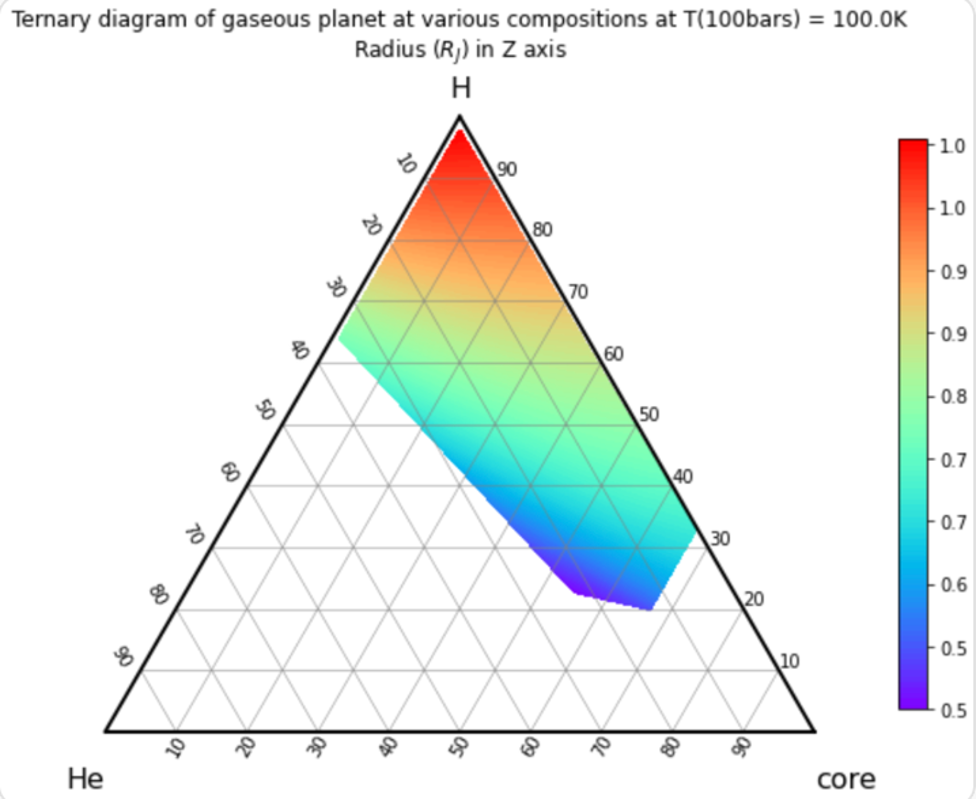
\includegraphics[width=0.48\textwidth]{Images/degeneracies.png}
    \caption{Degeneracy plot (ternary plot), representing radius ($R_J$) at various, hydrogen, helium and core mass fractions}
    \label{fig:Degen}
\end{figure}

\section{Notes on exorem model selection}

As stated in the model description, exorem can in certain conditions struggle to converge. This happens generally in zones of the grid where the irradiation temperature is low and internal temperature high. Exorem can not balance the two stream flux model and balance the temperature at the bottom and top of the atmosphere. To deal with this, we help Exorem converge either by relying on T. Guillot (2010) \parencite{guillot_radiative_2010} non grey analytical model to provide initial pressure temperature profiles to guide exorem, these do not take into account irradiation. We can also re-inject profiles from the grid into Exorem, to accomplish this we find the closest profile to the given input parameters. However often this does not suffice and we still have non-converged profiles. It would be taking a risk to leave these profiles in the grid especially taking into account that for the moment we do not use any smoothing in the interpolation methods considered above. As such we chose to remove these profiles. Through trial and error it was shown that a systematic code to identify bad profiles was inefficient. As such a simple tree based model was used to identify such profiles. To do this a LGBM classifier was trained. LGBM classifiers are gradient boosted tree based learning algorithms that have low memory usage and are more efficient than most other classifiers such as random forests. They use leaf wise tree growth which increases efficiency. The disadvantage of such classifiers are that they are very sensitive to over-fitting and require relatively large data-sets. The model was trained using the top atmosphere flux ratio, bottom atmosphere flux ratio, effective temperature ratio, internal temperature and irradiation temperature. The more data science orientated reader might be concerned when seeing that dimensional data was used as a feature. We allowed ourselves to do this as the internal temperature and irradiation temperature are bounded by the grid limits, rigorously one should divide these values by their maximum value on the grid. The results obtained were an accurate categorisation of 98\% of profiles, with an equal split percentage wise between false positives and false negatives. 

\section{Notes on entropy of mixes}

As shown in \parencite{chabrier_new_2019}, the expression for a given extensive quantity $W$ at a given $(T,P)$ for a mixture is given by :

\begin{align} 
    W(T,P) = \sum_{i} X_{i} W_{i}(T,P)
    \label{eq:extensive_qty}
\end{align}

With :

\begin{align} 
    X_{i} = \frac{M_i}{\sum_{i}M_{i}}
    \label{eq:mass_fraction}
\end{align}

Subsequently we can express the entropy of a mix of $He/H/H_2O$ as follows :

\begin{align} 
    S = \sum_{i} X_{i} S_{i}(T,P) + S_{mix}(T,P)
    \label{eq:entropy_mix1}
\end{align}

\begin{align} 
    S = X_{H} S_{H}(T,P) + X_{He} S_{He}(T,P) \nonumber \\ 
    + X_{H_2O} S_{H_2O}(T,P) + S_{mix}(T,P)
    \label{eq:entropy_mix2}
\end{align}

With here $S_{mix}(T,P)$ the ideal mixing term that we will better define subsequently. But we shall consider equal to zero.

We need to substitute the expressions for the mass fractions.                            % Comment out to exclude appendix

\end{document}

